\documentclass[xcolor=table]{beamer}
\usetheme{default}
\definecolor{darkscarlet}{rgb}{0.34, 0.01, 0.1}
\usecolortheme{default}
\usecolortheme[named=darkscarlet]{structure}
\setbeamercolor{title}{bg=white, fg=darkscarlet}
\definecolor{cerise}{rgb}{0.87, 0.19, 0.39}
\hypersetup{colorlinks=TRUE,linkcolor=cerise,urlcolor=cerise, citecolor=cerise}

% nummering

\setbeamertemplate{caption}[numbered]

% taal

% tekens
\usepackage{fontspec}
\usefonttheme{serif}
\setmainfont[BoldFont=brillb.ttf, ItalicFont=brilli.ttf, BoldItalicFont=brillbi.ttf]{brill.ttf}

% tekst doorstrepen, kennelijk heb je daar een apart pakket voor nodig

\usepackage[normalem]{ulem}

% plaatjes

\usepackage{graphicx}
\usepackage{subfig}

% tabellen

\usepackage{multirow}

% voorbeelden

\usepackage{philex}
\usepackage{forest}

% glossen

\usepackage{leipzig}
\newleipzig{hab}{hab}{habitual}
\newleipzig{aor}{aor}{aorist}
\makeglossaries

% bibliography

\usepackage[backend=biber,
        bibstyle=biblatex-sp-unified,
        citestyle=sp-authoryear-comp,
        doi=false,
        maxcitenames=3,
        maxbibnames=99]{biblatex}
\addbibresource{bibliography.bib}


% custom footline

\setbeamerfont{footline}{size=\fontsize{20}{20}\selectfont}

\newcommand{\Ffootline}{\footnotesize
\insertsection
\hfill
\href{https://github.com/agricolamz/2020.03.24_NIS_dictionaries}{github/agricolamz/2020.03.24\_NIS\_dictionaries}
\hfill
\insertframenumber/\inserttotalframenumber} 

% custom footline deel 2

\setbeamertemplate{footline}{%
\usebeamerfont{structure}
\begin{beamercolorbox}[wd=\paperwidth,ht=2.25ex,dp=1ex]{title in head/foot}%
\Tiny\hspace*{4mm} \Ffootline \hspace{4mm}
\end{beamercolorbox}}

% navigatiesymbolen uitzetten

\beamertemplatenavigationsymbolsempty
 
 
% titelpagina 

\title{Phonological and morphological variation in Botlikh: \\ Comparing two dictionaries}
\author{George Moroz, Chiara Naccarato, Samira Verhees \\
Linguistic Convergence Laboratory, NRU HSE}
\date{24.03.2020}

% links

\usepackage{hyperref}

%\newcommand\pro{\item[$+$]}
%\newcommand\con{\item[$-$]}

% ž š šč č ` 

\begin{document}

\begin{frame}
\titlepage
\end{frame}

\section{Introduction}
\begin{frame}{Botlikh}
    \begin{itemize}
        \item Botlikh < Andic < Avar-Andic-Tsezic < East Caucasian
        \item Spoken by \textasciitilde{}5,000-8,000 speakers
        \item Three villages in the Botlikh district of the Republic of Daghestan: Botlikh, Miarso, and Ashino
        \item Unwritten and mostly spoken at home; the Cyrillic script of Avar functions as an ad hoc writing system on social media
        \item Evaluated as ``threatened'' by Ethnologue \citep{simonsfenning2018}, but many children still speak the language and attitudes are positive
        \item Heavy influence from Avar and Russian 
    \end{itemize}
\end{frame}

\begin{frame}{Botlikh}
\begin{figure}[h]
\centering
\fbox{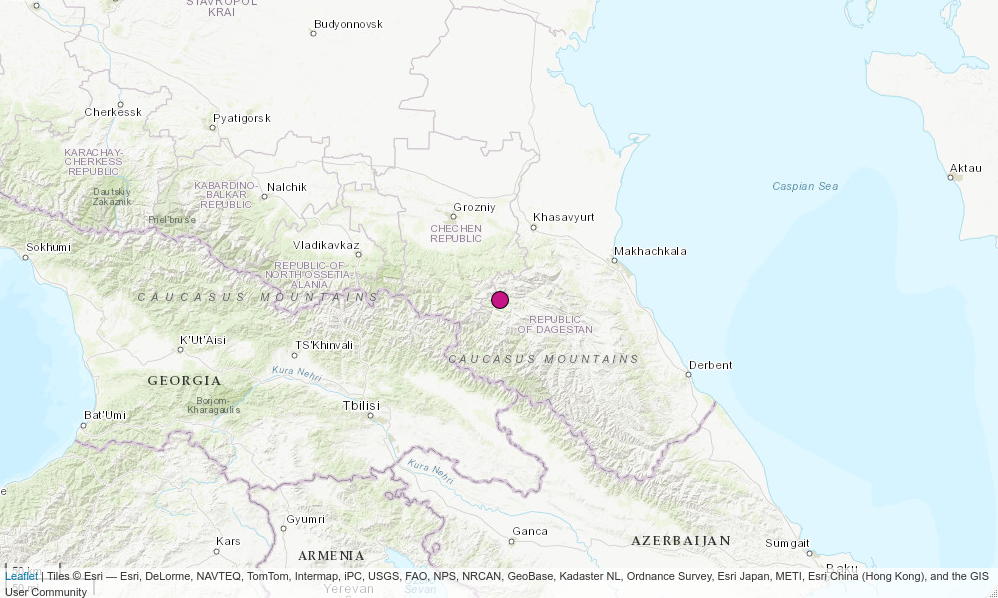
\includegraphics[scale=0.4]{images/globalmap.png}}
\caption{Botlikh on the map}
\end{figure}
\end{frame}

\begin{frame}{Botlikh literature}
\begin{itemize}
    \item One full reference grammar in Georgian \citep{gudava1962}
    \item Several short sketches mostly based on information contained in the grammar by Togo E. Gudava \citep{gudava1967, azaev2000, saidova2001, magomedbekova2001, xalidova2017, alekseevverhees}
    \item Several works on the lexicon and word formation \citep{azaev1975, sulejmanova2013, alekseev2016}
    \item In general poorly described compared to other Andic languages like Godoberi or Bagvalal, BUT two Botlikh-Russian dictionaries are available to date \citep{saidovaabusov2012, alekseev2019}
\end{itemize}
\end{frame}

\begin{frame}{Two dictionaries}
\begin{figure}[h]
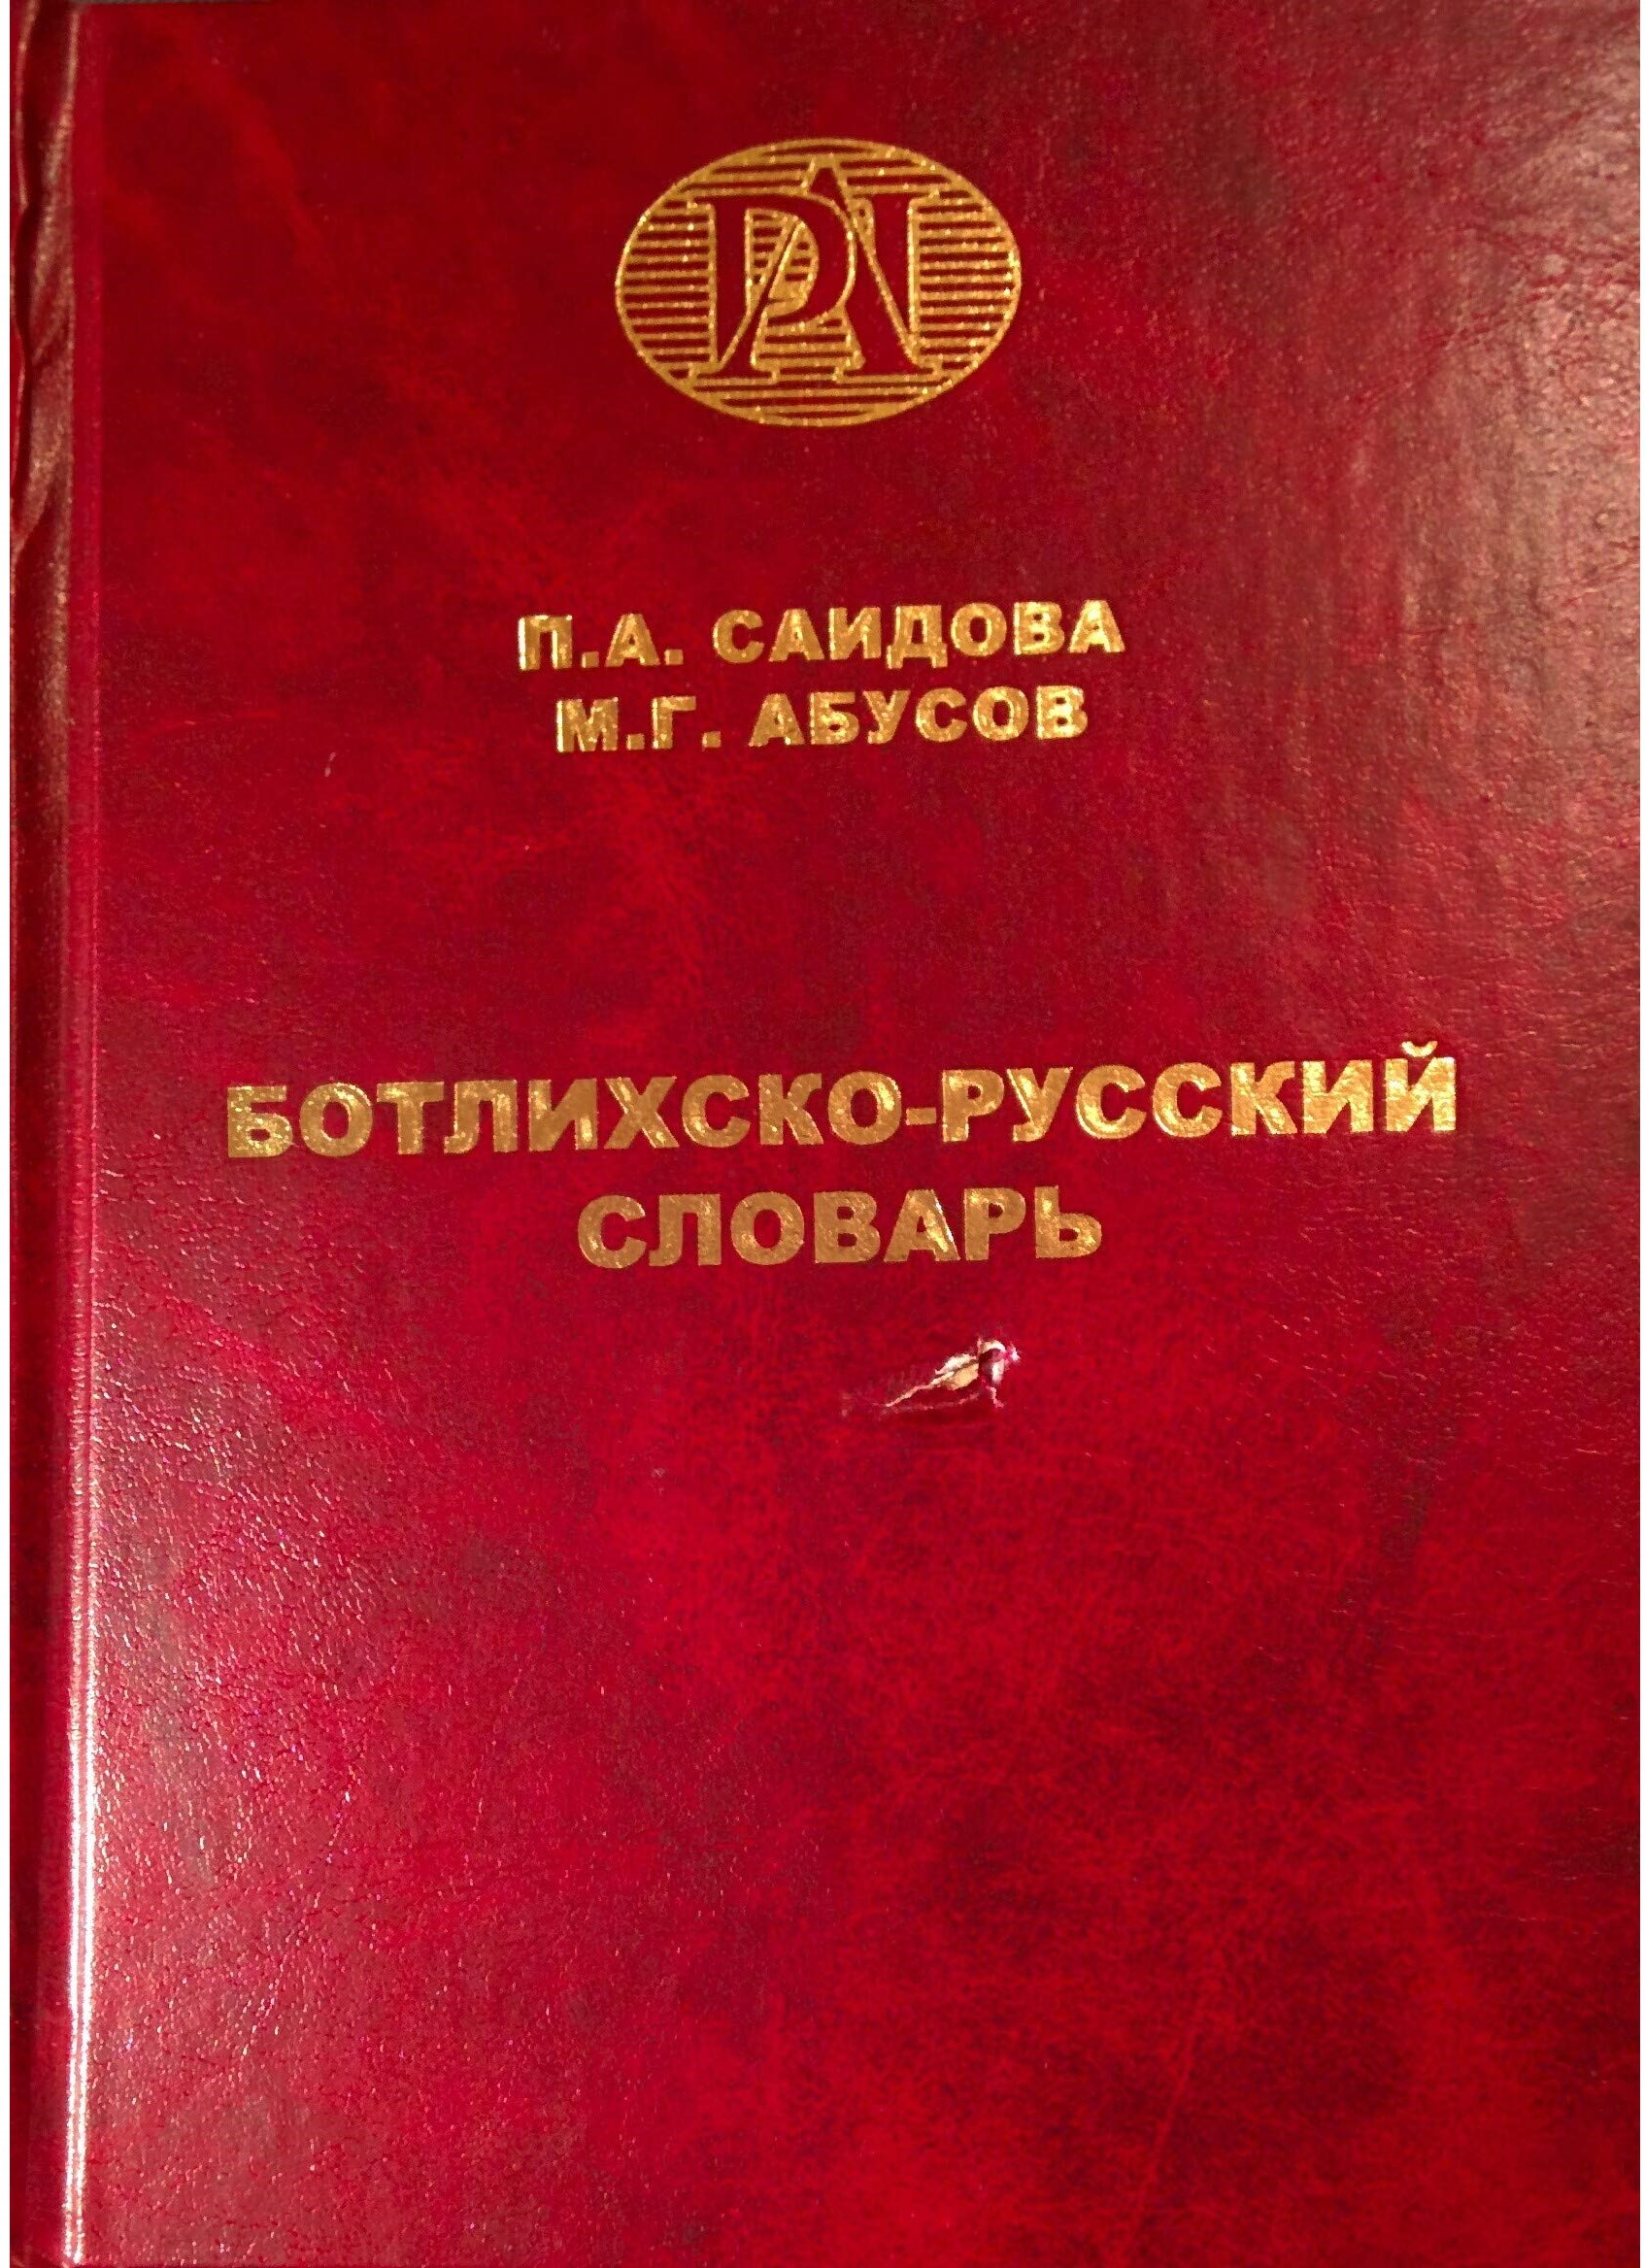
\includegraphics[height=6cm]{images/abusov2012.jpg} 
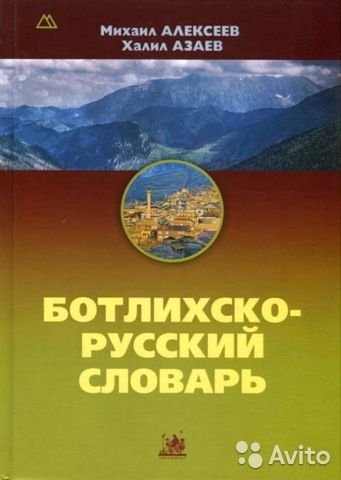
\includegraphics[height=6cm]{images/alekseev2019.jpg}
\label{two_dicts}
\caption{Two Botlikh-Russian dictionaries}
\end{figure}
\end{frame}

\begin{frame}{Two dictionaries}
\begin{itemize}
    \item \citet{saidovaabusov2012} compiled in the 2000s by a native speaker of Botlikh (Magomed G. Abusov) and an experienced linguist (Patimat A. Saidova)
    \item \citet{alekseev2019} compiled in the 1960s/1970s by a native speaker of Botlikh and philologist (Xalil G. Azaev), later (in the 2000s) systematized by an experienced linguist (Mixail E. Alekseev), and published posthumously after the editing by Timur A. Maisak
\end{itemize}
\end{frame}

\begin{frame}{Two dictionaries}
\begin{itemize}
    \item Comparable both quantitatively and qualitatively
    \item \textasciitilde{}8,000 headwords for \citet{saidovaabusov2012} vs. \textasciitilde{}9,000 words and expressions for \citet{alekseev2019}
    \item Although the data in \citet{alekseev2019} were collected several decades earlier, Magomed G. Abusov also consulted elderly speakers with the aim of collecting archaic vocabulary 
    \item \citet{saidovaabusov2012} also contains some notes on Miarso; reference to Miarso variants is not explicit in \citet{alekseev2019}, but it seems that such variants are occasionally reported in this dictionary too
    \item No metadata on the speakers consulted
    \item At first glance, the two resources seemed to display variation
\end{itemize}
\end{frame}

\begin{frame}{Our research}
\begin{itemize}
    \item Comparison of the two resources
    \item A unique opportunity to conduct a quantitative investigation of an understudied language
    \item Provide numerical approximations for the impressionistic observations available in the existing literature
    \item Analysis of both phonological and morphological features 
    \item Detect patterns of systematic variation within these two areas
\end{itemize}
\end{frame}

\begin{frame}{Outline}
\begin{itemize}
    \item Data 
    \begin{itemize}
        \item merging
        \item extracting grammatical information
        \item pairing and annotation
    \end{itemize}
    \item Analysis
    \begin{itemize}
        \item phonology (George Moroz)
        \item nominal morphology (Chiara Naccarato)
        \item verbal morphology (Samira Verhees)
    \end{itemize}
    \item Results and discussion
    \item Methodological remarks 
\end{itemize}
\end{frame}

\section{Data}
\begin{frame}{Merging (George Moroz)}
\begin{figure}[h]
\centering
\fbox{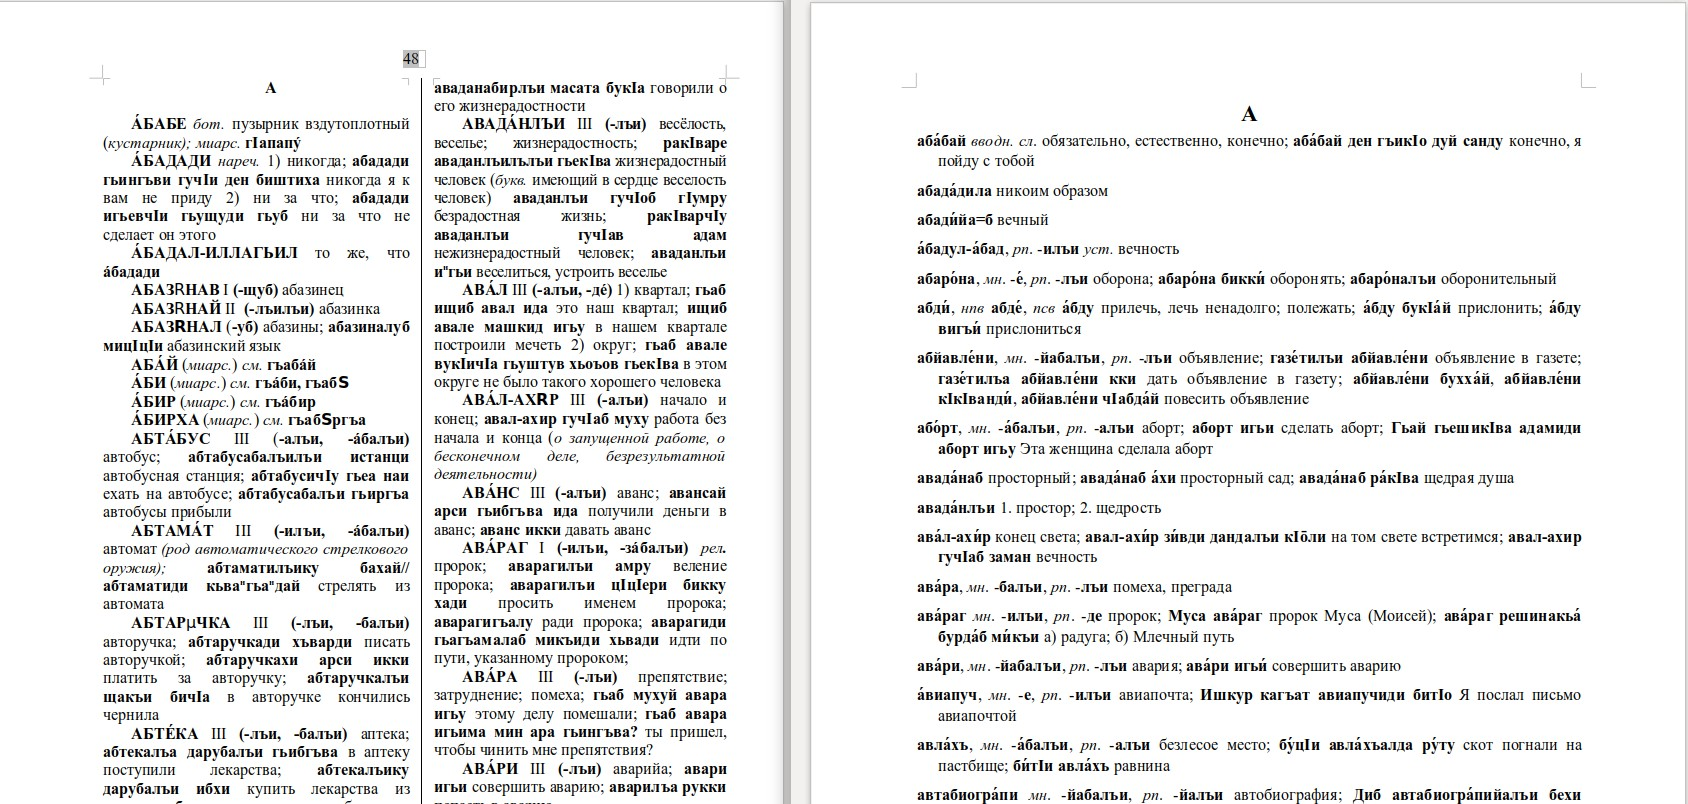
\includegraphics[scale=0.17]{images/dicts.jpg}}
\caption{Merging the dictionaries}
\end{figure}
\end{frame}

\begin{frame}{Merging (George Moroz)}
From two .doc files to one .xls:
\begin{itemize}
    \item .doc preprocessing: convert files to .html, change non-standard symbols, solve several tag problems (I, $^\text{H}$, etc.)
    \item extract first bold entrance, parse parenthesis for grammar information
\end{itemize}
\end{frame}

\begin{frame}{Extracting grammatical information}
\begin{itemize}
    \item Total number of lexemes extracted: 8,464 from \citet{saidovaabusov2012} and 6,821 from \citet{alekseev2019}
    \item Nouns: 2,871 from \citet{saidovaabusov2012} and 3,097 from \citet{alekseev2019}
    \begin{itemize}
        \item grammatical information: genitive and plural
    \end{itemize}
    \item Verbs: 1,504 from \citet{saidovaabusov2012} and 1,640 from \citet{alekseev2019}
    \begin{itemize}
        \item grammatical information: habitual and aorist
    \end{itemize}
\end{itemize}
\end{frame}

\begin{frame}{Extracting grammatical information}
\begin{figure}[h]
\centering
\fbox{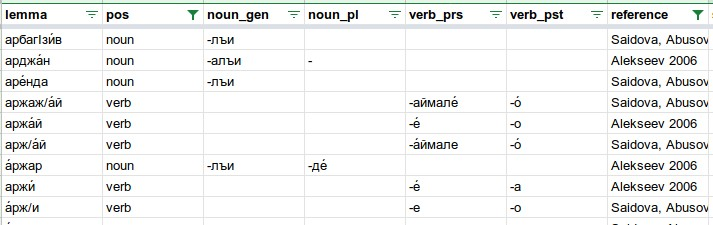
\includegraphics[scale=0.4]{images/table.jpg}}
\caption{The database}
\end{figure}
\end{frame}

\begin{frame}{Pairing}
We manually checked for lexemes represented in both dictionaries to carry out phonological and morphological analysis 
\begin{figure}[h]
\centering
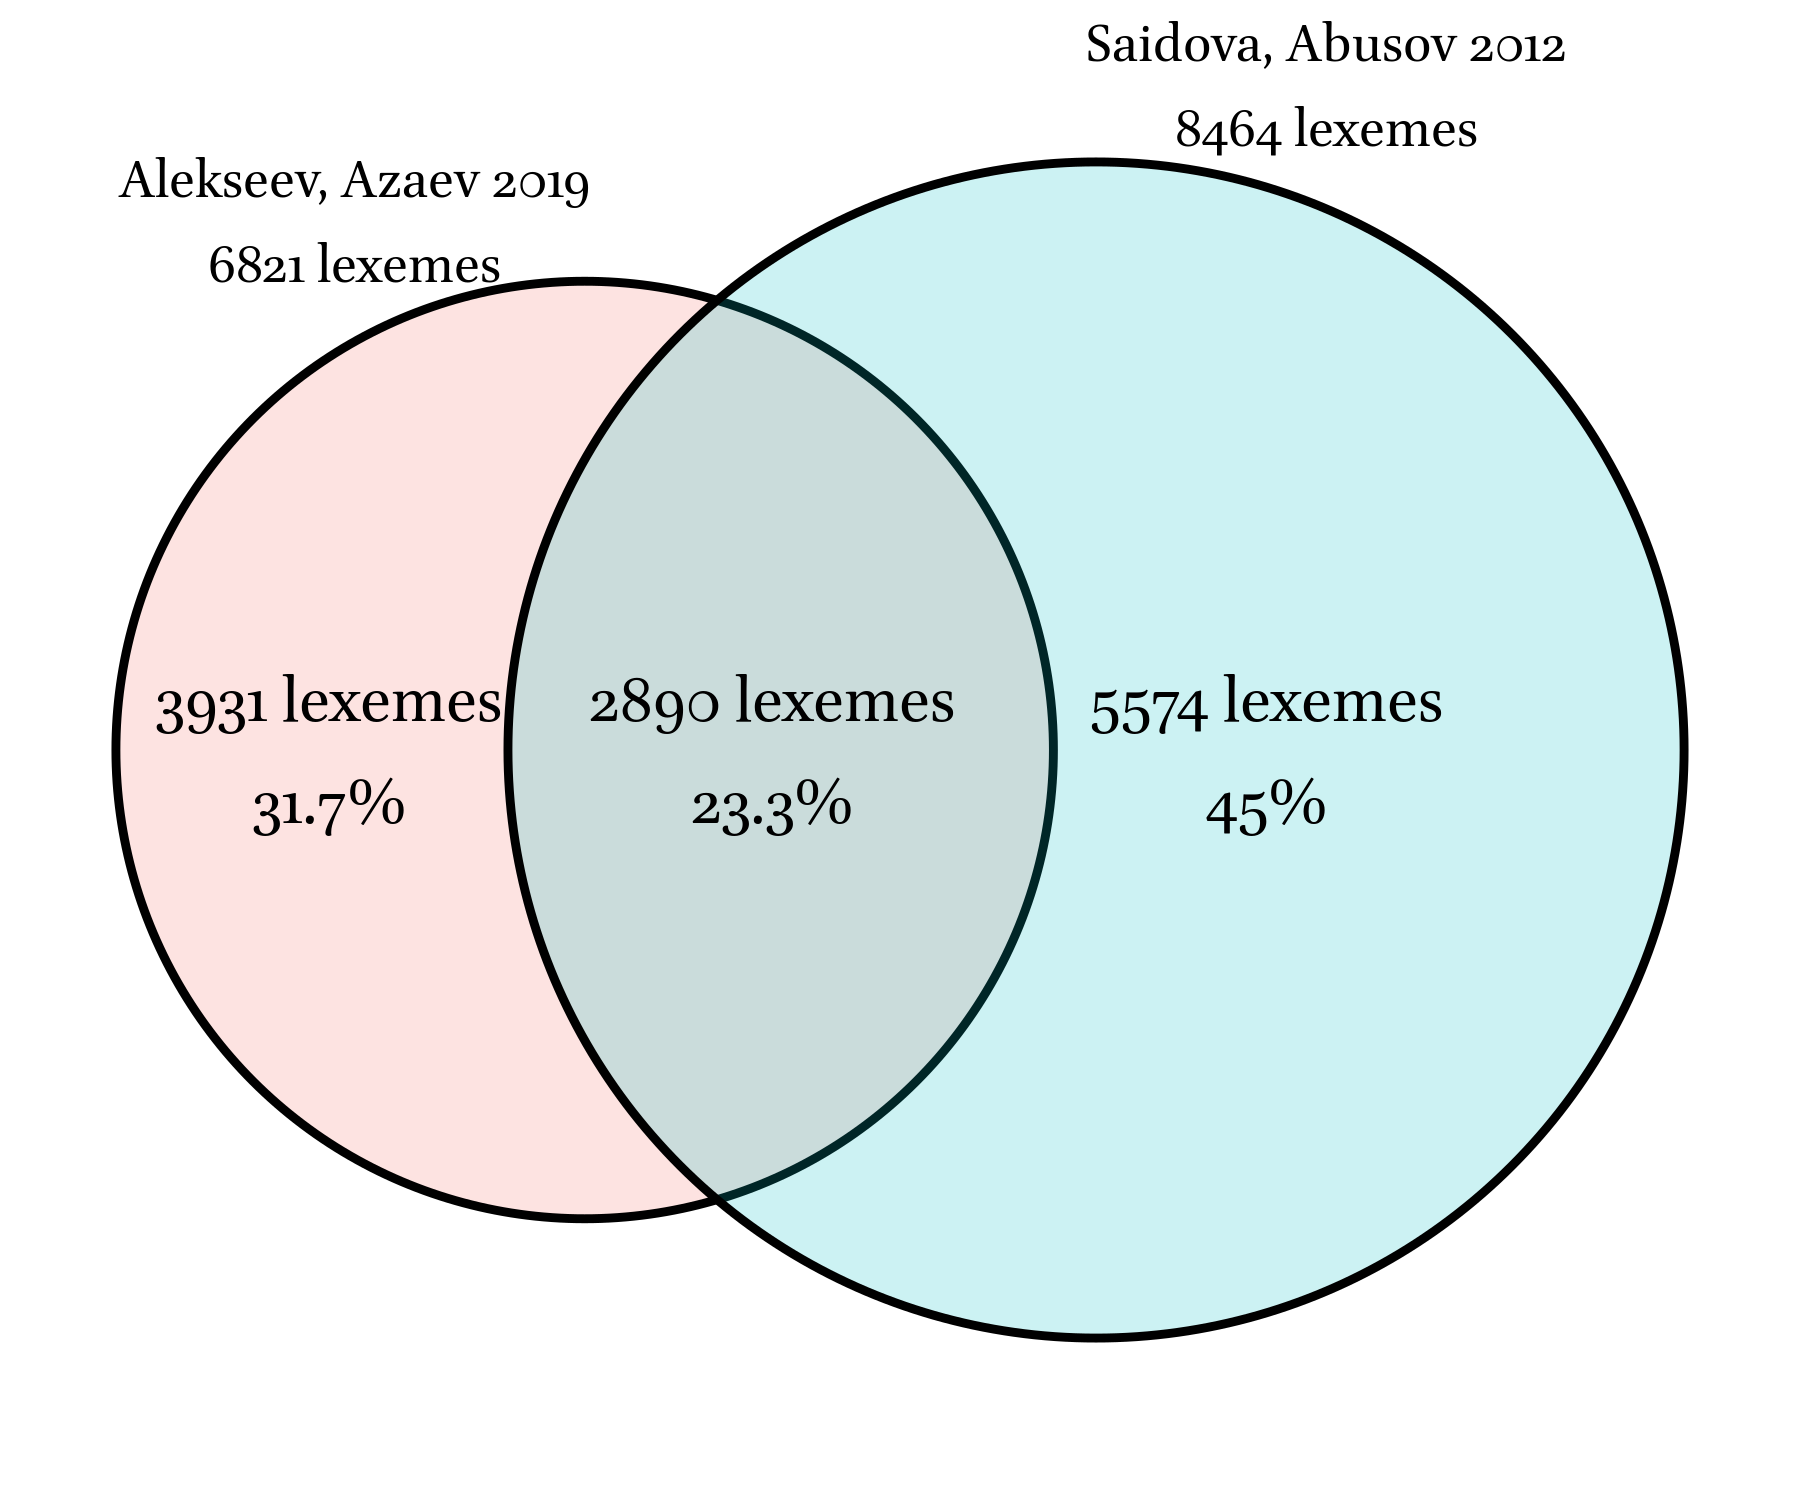
\includegraphics[scale=0.45]{images/venn.png}
\caption{The database}
\end{figure}
\end{frame}

\begin{frame}{Pairing}
We manually checked for lexemes represented in both dictionaries to carry out phonological and morphological analysis 
\begin{itemize}
    \item Those 2,890 include all POS
    \item There are multiple entries for the same root \\
    \citet{alekseev2019}: \textit{besqχe} `behind',  \textit{besqχéku }`from behind', \textit{besqé-ssu-b} `back/hind (adjective)', \textit{héči besqérussubla}`in the end'
    \item There are also some sayings and proverbs (about 670) that constitute separate entries in \citet{alekseev2019}\\
    \textit{héči besqχérussubla}
    `in the end'
\end{itemize}
\end{frame}

\begin{frame}{Annotation}
\begin{itemize}
    \item Manual correction of automatically extracted information about grammatical features
    \item Addition of further annotation (for features that appeared to be potentially relevant for our research):
    \begin{itemize}
        \item masdars
        \item borrowings
    \end{itemize}
    \item (In progress) Filter out superfluous entries for multi-word expressions and inflected forms
\end{itemize}
    
\end{frame}

\section{Phonology: segments}
\begin{frame}{Phonology}
\begin{itemize}
    \item There are 1,996 lexemes which look phonetically the same, while 909 are different (31\%)
    \item If we remove the stress sign, there are 2,449 lexemes which look phonetically the same, and 456 are different (16\%)
    \item[⇒] 15\% of lexemes have different stress pattern?.. \pause Yes, but including 265 (9\%) cases where the stress is present in one dictionary and absent in the other
\end{itemize}    
\end{frame}

\begin{frame}{Phonology}
\begin{itemize}
    \item What causes the difference between the two dictionaries?
    \begin{itemize}
        \item Stress pattern differences in 188 lexemes (about 6\%)
        \item Multiple cases where there is a small difference that could be explained either as a typo or in terms of phonological variation: \textit{čuhí} ‘to run’ [aa] vs. \textit{čũhí} [sa], \textit{kusu} ‘cherry plum’ [aa] vs. \textit{kussu} [sa]
        \item Multiple cases where Russian borrowings were adopted differently: \textit{a\textbf{w}tobus} ‘bus’ [aa] vs. \textit{a\textbf{b}tabus} [sa], \textit{bit\textbf{o}n} ‘milk can’ [aa] vs. \textit{bit\textbf{u}n} [sa], \textit{a\textbf{p}teka} ‘pharmacy’ [aa] vs. \textit{a\textbf{b}teka} [sa]
        \item Morphological preferences: \textit{dinija=\textbf{w}} ‘pious’ [aa] vs. \textit{dinija=\textbf{b}} [sa]
    \end{itemize}
\end{itemize}
\end{frame}

\begin{frame}{Phonology: segments}
\begin{tabular}{lll}
\citet{alekseev2019} &\citet{saidovaabusov2012} & \\
\textbf{About 25 cases}: & & \\
\textit{ãha\textbf{\underline{j}}r}   & \textit{ãhar}   & 'message’        \\
\textit{beʒa\textbf{\underline{j}}r}   & \textit{beʒir}   & 'roasting’       \\
\textit{mik'ku\textbf{\underline{j}}r} & \textit{mik'ːur} & 'swallowing’     \\
\textit{reqχu\textbf{\underline{j}}r}  & \textit{reqχʷir} & 'fight’          \\
\textit{reʃku\textbf{\underline{j}}r}  & \textit{reʃkur}  & 'overnight stay’ \\
\textit{rikʷa\textbf{\underline{j}}r}  & \textit{rikʷar} & 'lighting’     \\ \hline
\textit{χwardar} & \textit{χwardir} & 'digging' \\
\textit{miʔar} & \textit{miʔar} & 'nose'\\ 
\dots & \dots & \dots \\ 
\textbf{About 6 cases}: & & \\
\textit{ʃːalaj} & \textit{ʃːallaj} & 'silt' \\
\textit{inuʕala} & \textit{inuʕalla} & 'everywhere' \\
\textit{ʕila} & \textit{ʕilla} & 'reason' \\
\dots & \dots & \dots \\
\end{tabular}
\end{frame}

\begin{frame}{Phonology: compare Botlikh segments}
\begin{figure}[h]
\centering
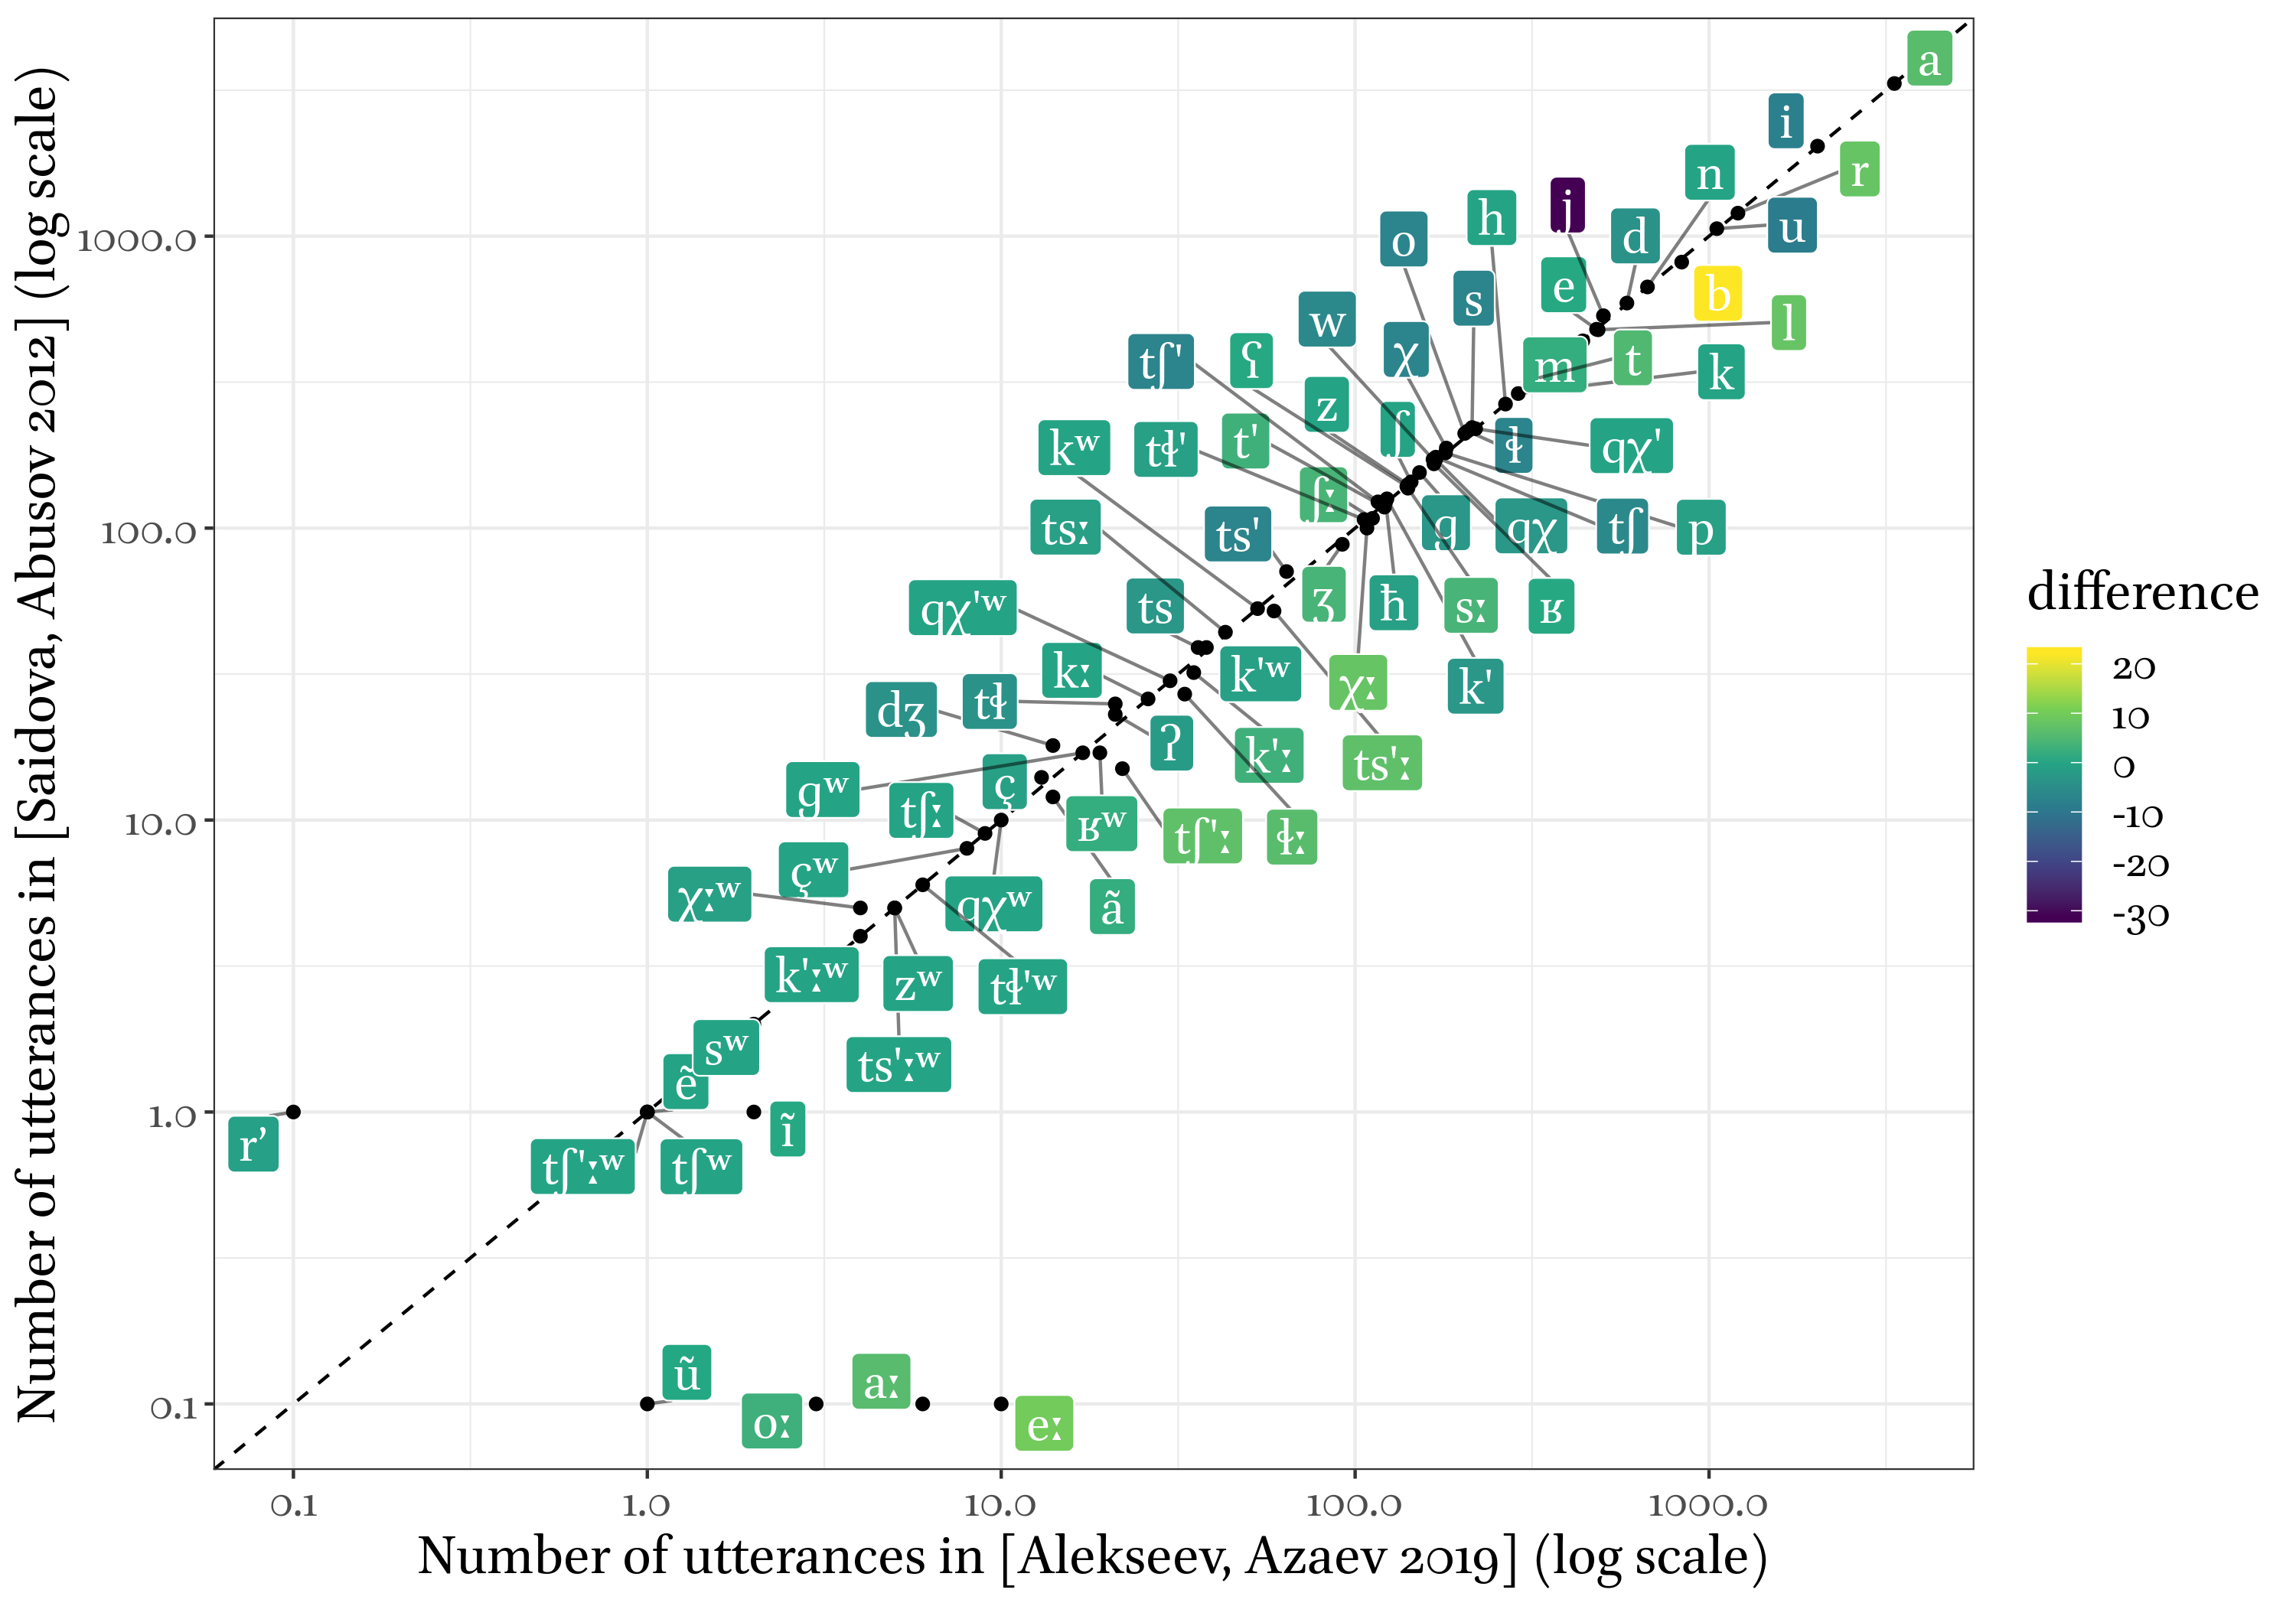
\includegraphics[width = \linewidth]{images/04_compare_botlikh_dicts_with_stress.png}
\end{figure}
\end{frame}

\begin{frame}{Phonology: compare Botlikh segments}
\begin{figure}[h]
\centering
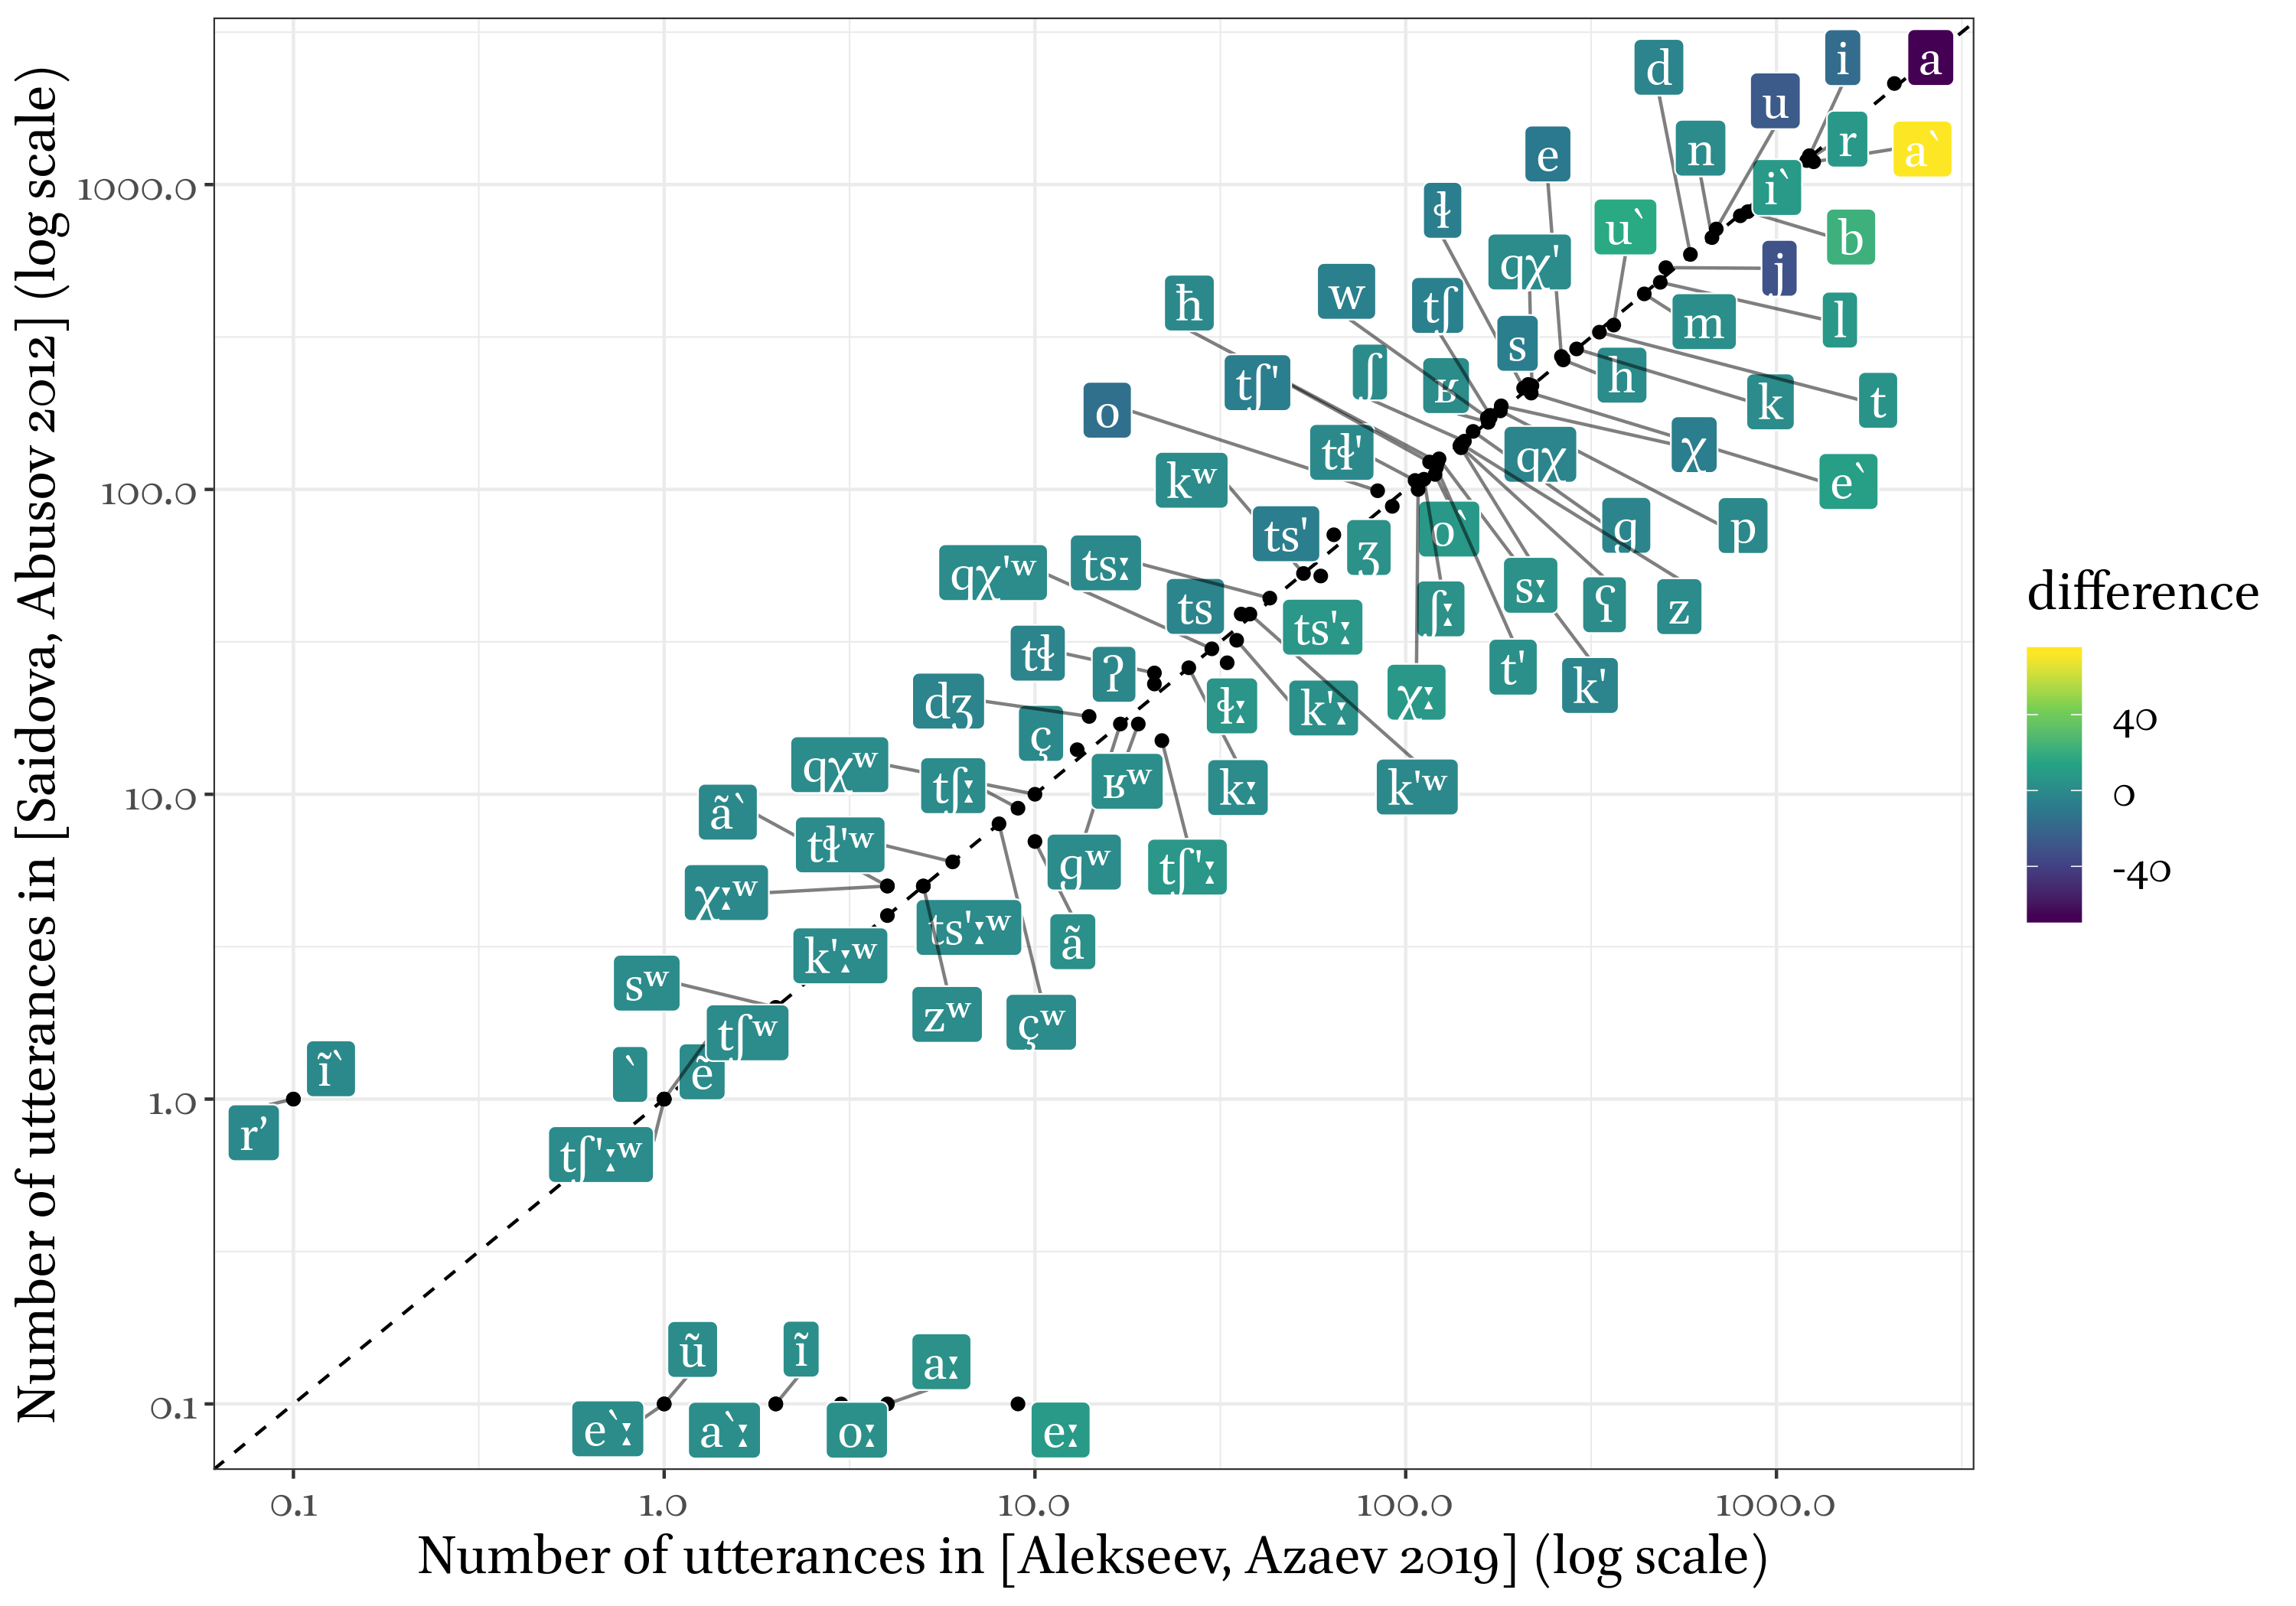
\includegraphics[width = \linewidth]{images/05_compare_botlikh_dicts_without_stress.png}
\end{figure}
\end{frame}

\begin{frame}{Zilo Andi data}

Dictionary data for Zilo were collected during fieldtrips to Zilo in 2016–2019 with N. Rochant, S. Verhees, A. Martynova and A. Zakirova who contributed to the same FieldWorks project

\begin{itemize}
    \item Contain morphological affixes
    \item Do not contain additional affixes in a lemma form
    \item Contain different stems of the same lexeme (e.g. \textsc{sg.abs, sg.obl, pl.abs, pl.obl, pst, npst}); those forms were removed during the analysis
    \item No information about stress
\end{itemize}

\end{frame}

\begin{frame}{Phonology: compare Botlikh and Zilo segments}
\begin{figure}[h]
\centering
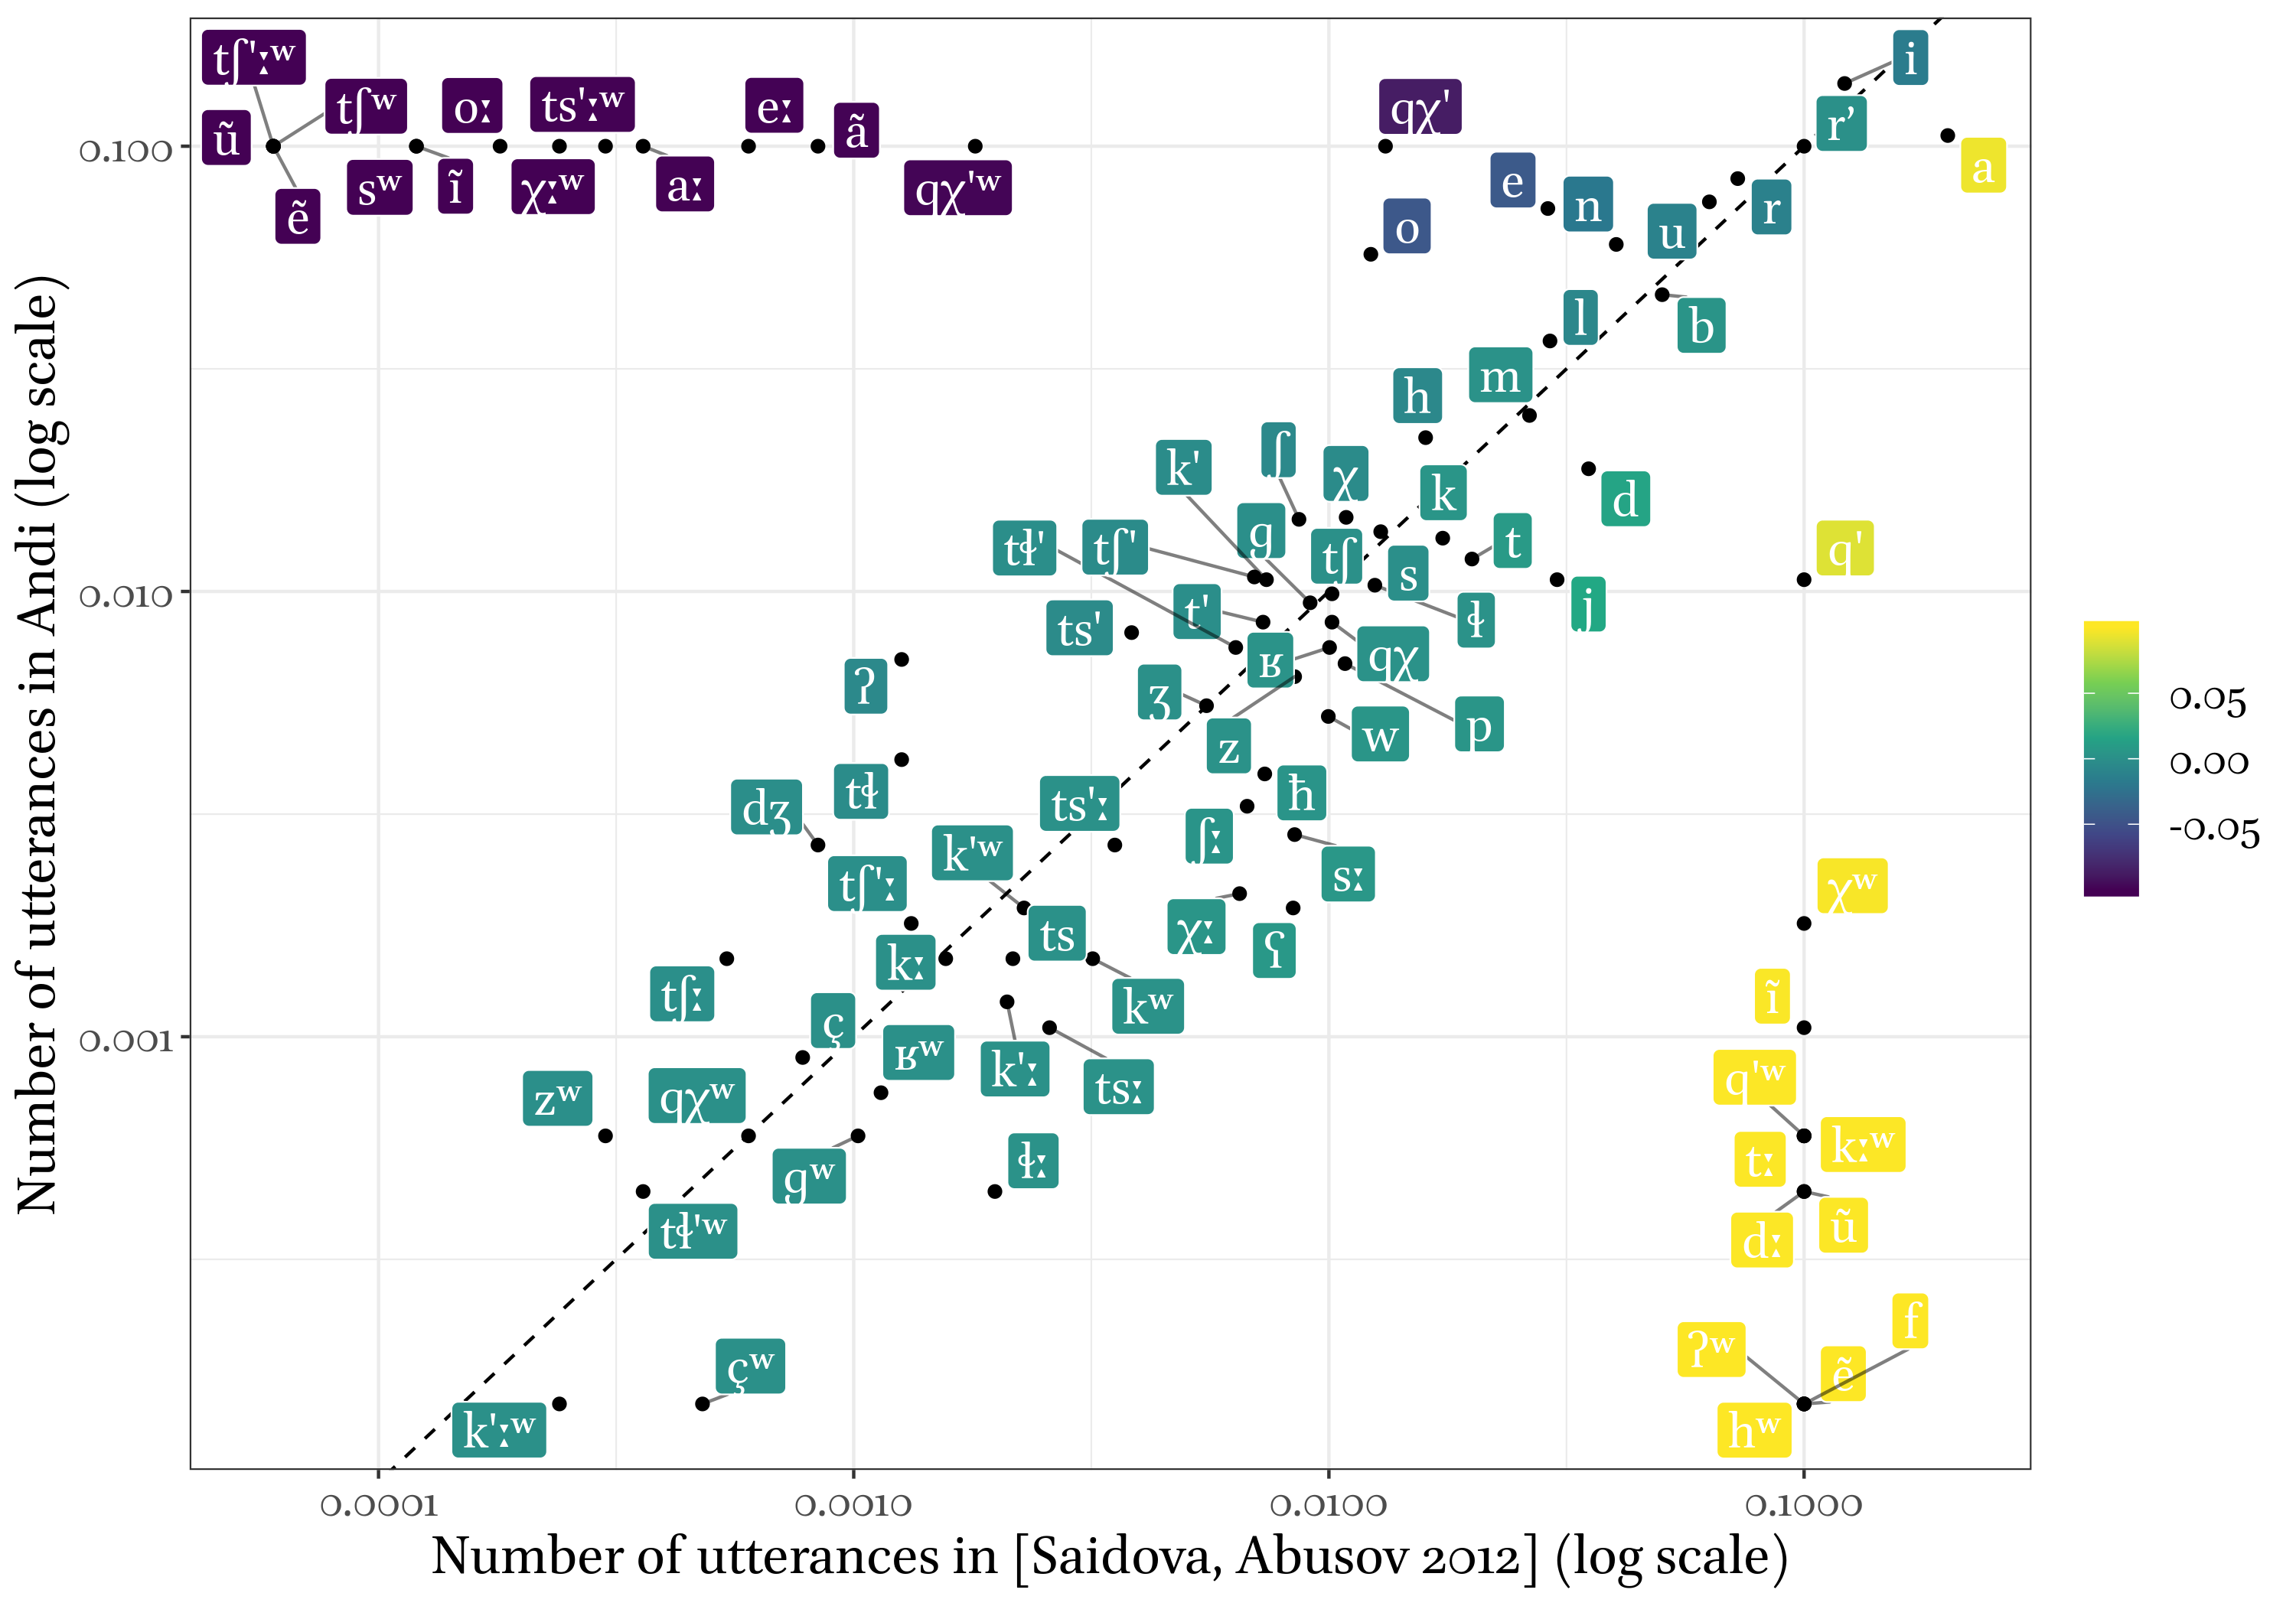
\includegraphics[width = \linewidth]{images/06_compare_botlikh_zilo.png}
\end{figure}
\end{frame}

\begin{frame}{Phonology: compare Botlikh and Zilo segments}
\begin{figure}[h]
\centering
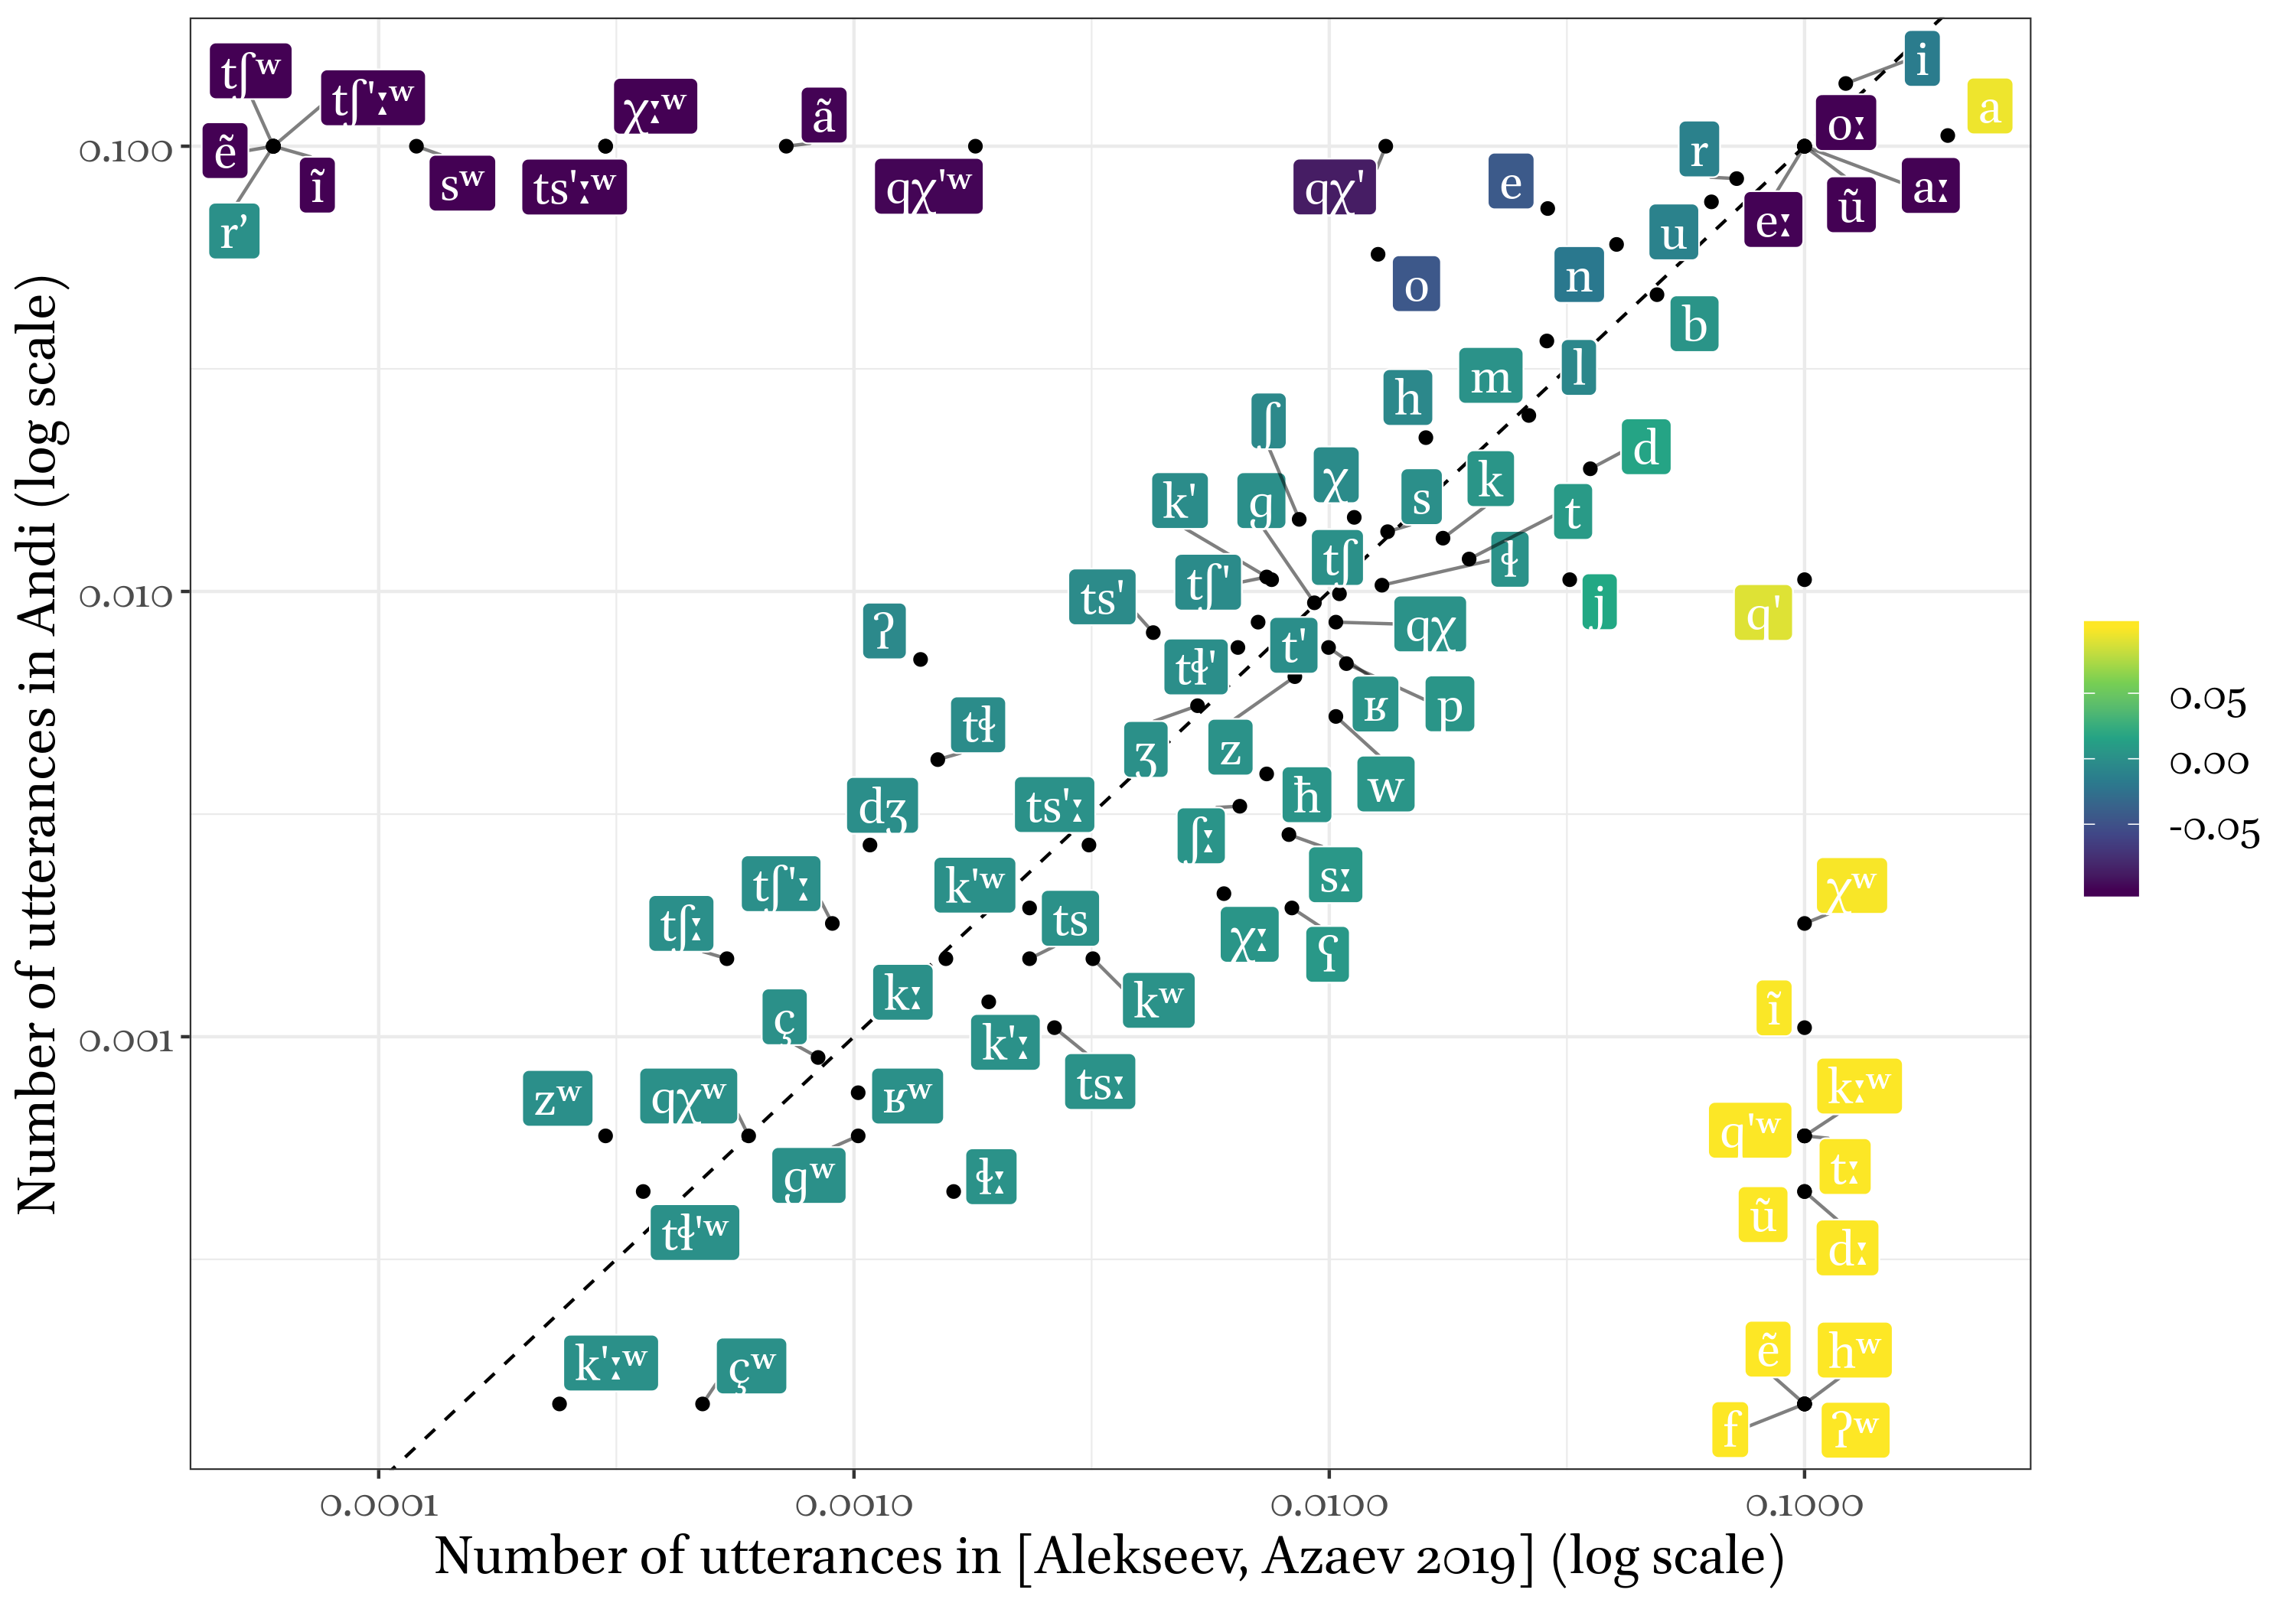
\includegraphics[width = \linewidth]{images/07_compare_botlikh_zilo.png}
\end{figure}
\end{frame}

\begin{frame}{Phonology: data--driven analysis of syllables}
\begin{forest}
[syllable, for tree={parent anchor=south, child anchor=north}
[onset [{[str}, tier = word]][rhyme [nucleus [e, tier = word]][coda [{ŋθ]}, tier = word]]]]]
\end{forest}

\begin{itemize}
    \item Analyze all onsets of initial syllables in the corpus
    \item Analyze all codas of final syllables in the corpus
    \item Generalize  obtained initials and codas into a syllable model
    \item Check, whether this model describes all intervocal consonant clusters
\end{itemize}
\end{frame}

\begin{frame}{Phonology: data--driven analysis of syllables}
\begin{figure}[h]
\centering
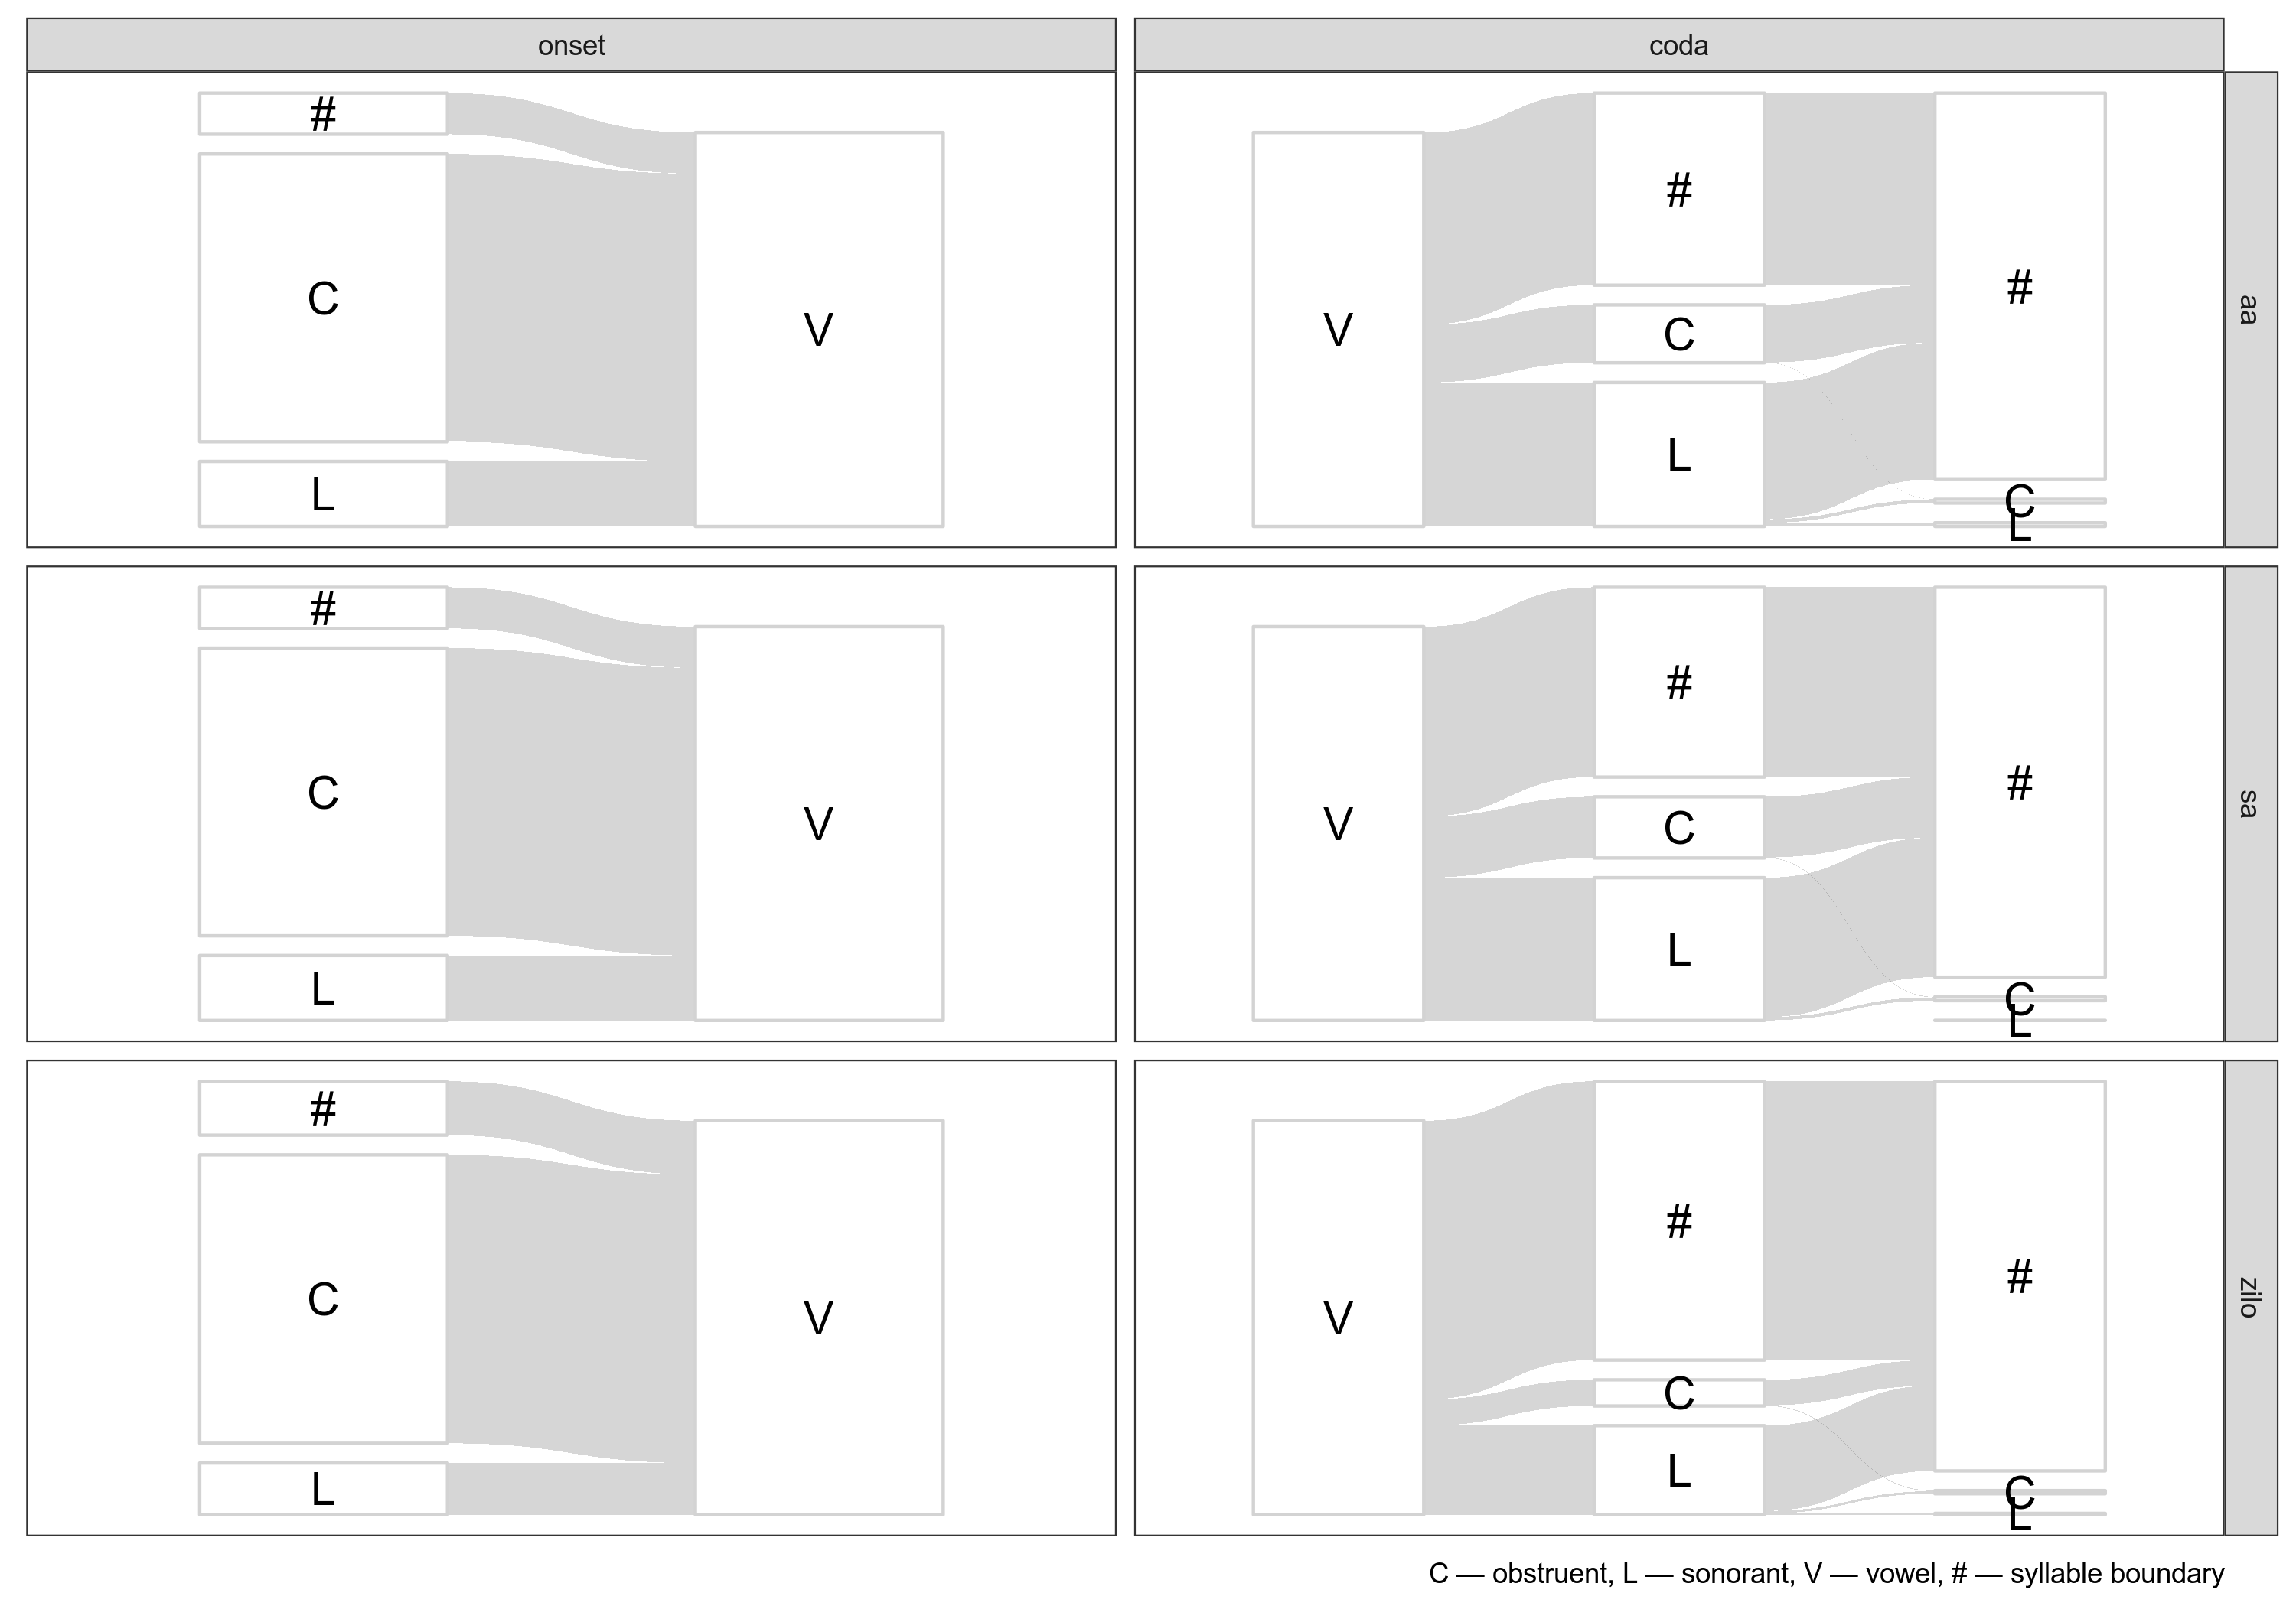
\includegraphics[width = \linewidth]{images/08_syllables.png}
\end{figure}
\end{frame}

\section{Nominal morphology}
\begin{frame}{Nominal morphology}
Two topics investigated:
\begin{itemize}
    \item Formation of the plural
    \begin{itemize}
        \item to check the productivity of different suffixes
    \end{itemize}
    \item Formation of the genitive
    \begin{itemize}
        \item to study alternations in the formation of oblique stems
    \end{itemize}
\end{itemize}
Comparison of the two resources to look for possible variation in such areas of nominal morphology \\ (based on 1,072 pairs retrieved during the first annotation round)
\end{frame}

\begin{frame}{Plural formation in Botlikh}
\begin{itemize}
    \item A suffix is attached to the absolutive stem: \\ \textit{na} `thing' < \textit{na-\textbf{baɬi}} `things'
    \item With stems ending in a consonant, the vowel \textit{-a-} is often inserted before the suffix: \\ \textit{majmalak}  `monkey' < \textit{majmalak-\textbf{a}-\textbf{baɬi}} `monkeys'
    \item With stems ending in a vowel, alternation can occur: \\ \textit{ruš\textbf{a}}  `tree' < \textit{ruš\textbf{i}-\textbf{baɬi}} `trees', \\ \textit{sal\textbf{u}}  `tooth' < \textit{sal\textbf{a}-\textbf{baɬi}} `teeth', \\ \textit{buraɬ\textbf{i}}  `pitcher' < \textit{buraɬ\textbf{a}-\textbf{baɬi}} `pitchers'
\end{itemize}
\end{frame}

\begin{frame}{Plural formation in Botlikh}
Among the most common suffixes are:
\begin{itemize}
    \item \textit{-baɬi} and allomorphs (\textit{-maɬi} for stems ending in a nasal, \textit{-wabaɬi} for stems ending in -\textit{u}, etc.), the variant \textit{-zabaɬi} (mostly with borrowings) \\ \textit{apicer} `officer' < \textit{apicer-\textbf{zabaɬi}} `officers'  
    \item \textit{-de} (mostly for stems ending in a sonorant) \\ \textit{ambur} `roof' < \textit{ambur-\textbf{de}} `roofs'
    \item \textit{-e} and its variant \textit{-we} (for stems ending in -\textit{u}) \\ \textit{čan} `deer' < \textit{čan-\textbf{e}} `deers'
\end{itemize}
Other, less common, suffixes are: -\textit{(b)daɬi}, -\textit{(b)diɬi}, -\textit{(a)l}, -\textit{rdi}, -\textit{bala(l)}
\end{frame}

\begin{frame}{Plural formation in Botlikh}
\centering
Can our dictionary data help us be more precise about the distribution/frequency/productivity of plural suffixes in Botlikh? \\ ... \\ Do the two dictionaries show any variation in these respects?
\end{frame}

\begin{frame}{Plural suffixes in the dictionaries}
\begin{itemize}
    \item Plural suffixes are not reported for all nouns, cf. \textit{singularia tantum} and plural entries (nationalities, \textit{pluralia tantum})
    \item Quite often more than one variant is reported
\end{itemize}
\begin{table}[]
\caption{Plural suffixes in the dictionaries}
\centering
\begin{tabular}{lcc}
          & \multicolumn{1}{l}{\textbf{Saidova \& Abusov (2012)}} & \multicolumn{1}{l}{\textbf{Alekseev \& Azaev (2019)}} \\
\textbf{-\textit{(x)baɬi}}  & 292                                          & 298                                          \\
\textbf{-\textit{de}}       & 128                                          & 354                                          \\
\textbf{-\textit{(w)e}}     & 141                                          & 239                                          \\
\textbf{other}     & 24                                           & 21                                           \\
\textbf{no plural} & 499                                          & 193                                         
\end{tabular}
\end{table}
\end{frame}

\begin{frame}{Plural suffixes in the dictionaries}
\begin{figure}[h]
\caption{Plural suffixes in the dictionaries}
\centering
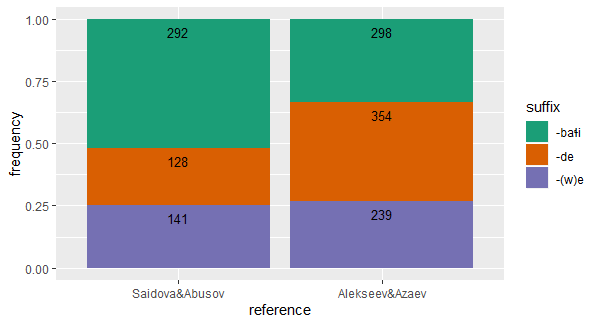
\includegraphics[height=5.5cm]{images/plural.png}
\end{figure}
\centering
\small (χ² = 47.118, df = 2, p-value = 5.869e-11)
\end{frame}

\begin{frame}{Plural suffixes in the dictionaries}
\begin{itemize}
    \item Preference for -\textit{(x)baɬi} over -\textit{de} in \citet{saidovaabusov2012} vs. the opposite trend in \citet{alekseev2019}
    \item The higher frequency of -\textit{de} in \citet{alekseev2019} is partly due to masdars
    \begin{itemize}
        \item \citet{saidovaabusov2012} almost never report the plural form for such nouns, whereas \citet{alekseev2019} consistently report -\textit{de}
    \end{itemize}
    % Try graph without masdars
    % geom_text(color = "white", size = 8)
    \item Variation often involves (but is not restricted to) borrowings
    \begin{itemize}
        \item \textit{birgadir} `foreman' < \textit{birgadir-\textbf{zabaɬi}} vs. \textit{birgadir-\textbf{de}}
        \item \textit{kassir} `cashier' < \textit{kassir-\textbf{zabaɬi}} vs. \textit{kassir-\textbf{de}}
    \end{itemize}
    \item The frequent mentioning of more than one variant might suggest idiosyncratic variation
\end{itemize}
\end{frame}

\begin{frame}{Case declension in Botlikh}
Two declension types
\begin{itemize}
    \item I type --- the stem does not change when a suffix is attached (mostly stems ending in a vowel and masdars) \\ \textit{bab\textbf{u}} `mom' < \textit{bab\textbf{u}-\textbf{ɬi}} (genitive) \\ \textit{masir} `measurement' < \textit{masir-\textbf{ɬi}} (genitive)  
    \item II type --- case suffixes are attached to the oblique stem of the noun (mostly stems ending in a consonant, sometimes stems ending in a vowel) \\ \textit{askar} `army' < \textit{askar-\textbf{a}-\textbf{ɬi}} (genitive) \\ \textit{din} `religion' < \textit{din-\textbf{i}-\textbf{ɬi}} (genitive) \\ \textit{ima} `father' < \textit{im\textbf{u}-\textbf{ɬi}} (genitive) 
\end{itemize}
\end{frame}

\begin{frame}{Case declension in Botlikh}
\centering
Can our dictionary data help us be more precise about the patterns of case declension (oblique stem formation) and their frequencies? \\ ... \\ Do the two dictionaries show any variation in these respects?    
\end{frame}

\begin{frame}{Oblique stem formation in the dictionaries}
We used the grammatical information included in the dictionaries (genitive suffix) to investigate oblique stem formation in Botlikh
\begin{table}[]
\caption{Oblique stem formation in the dictionaries}
\centering
\begin{tabular}{|c|c|c|c|c|c|c|c|c|}
\hline
            & \multicolumn{2}{c|}{\textit{-ɬi}}                       & \multicolumn{2}{c|}{\textit{-\textbf{a}-ɬi}}                                       & \multicolumn{2}{c|}{\textit{-\textbf{i}-ɬi}}                                       & \multicolumn{2}{c|}{\textit{-\textbf{u}-ɬi}}                   \\ \hline
consonant   & {\color[HTML]{1B9045} 232} & {\color[HTML]{CE6301} 266} & {\color[HTML]{1B9045} \textbf{228}} & {\color[HTML]{CE6301} \textbf{167}} & {\color[HTML]{1B9045} \textbf{104}} & {\color[HTML]{CE6301} \textbf{141}} & {\color[HTML]{1B9045} -}  & {\color[HTML]{CE6301} 1}  \\ \hline
\textit{-a} & {\color[HTML]{1B9045} 182} & {\color[HTML]{CE6301} 167} & {\color[HTML]{1B9045} -}            & {\color[HTML]{CE6301} -}            & {\color[HTML]{1B9045} \textbf{3}}   & {\color[HTML]{CE6301} \textbf{13}}  & {\color[HTML]{1B9045} 15} & {\color[HTML]{CE6301} 14} \\ \hline
\textit{-i} & {\color[HTML]{1B9045} 143} & {\color[HTML]{CE6301} 151} & {\color[HTML]{1B9045} \textbf{10}}  & {\color[HTML]{CE6301} \textbf{4}}   & {\color[HTML]{1B9045} -}            & {\color[HTML]{CE6301} -}            & {\color[HTML]{1B9045} 3}  & {\color[HTML]{CE6301} 2}  \\ \hline
\textit{-u} & {\color[HTML]{1B9045} 81}  & {\color[HTML]{CE6301} 78}  & {\color[HTML]{1B9045} 1}            & {\color[HTML]{CE6301} -}            & {\color[HTML]{1B9045} -}            & {\color[HTML]{CE6301} 3}            & {\color[HTML]{1B9045} -}  & {\color[HTML]{CE6301} -}  \\ \hline
\textit{-e} & {\color[HTML]{1B9045} 6}   & {\color[HTML]{CE6301} 6}   & {\color[HTML]{1B9045} -}            & {\color[HTML]{CE6301} -}            & {\color[HTML]{1B9045} -}            & {\color[HTML]{CE6301} -}            & {\color[HTML]{1B9045} -}  & {\color[HTML]{CE6301} -}  \\ \hline
\textit{-o} & {\color[HTML]{1B9045} 7}   & {\color[HTML]{CE6301} 7}   & {\color[HTML]{1B9045} -}            & {\color[HTML]{CE6301} -}            & {\color[HTML]{1B9045} -}            & {\color[HTML]{CE6301} -}            & {\color[HTML]{1B9045} -}  & {\color[HTML]{CE6301} -}  \\ \hline
\end{tabular}
\end{table}
\centering
\small {\color[HTML]{1B9045} Saidova \& Abusov (2012)} vs. {\color[HTML]{CE6301} Alekseev \& Azaev (2019)}
\end{frame}

\begin{frame}{Oblique stem formation in the dictionaries}
\begin{figure}[h]
\centering
\caption{Oblique stem formation for stems ending in a consonant}
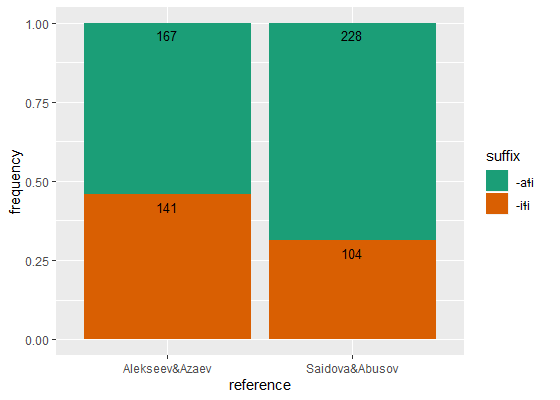
\includegraphics[height=5.5cm]{images/genitive.png}
\end{figure}
\centering
\small (χ² = 13.523, df = 1, p-value = 0.0002357)
\end{frame}

\begin{frame}{Oblique stem formation in the dictionaries}
\begin{itemize}
    \item Significant variation between the two dictionaries in the formation of oblique stems for nouns ending in a consonant
    \item This again involves (but is not restricted to) borrowings (a general preference for -\textit{a}- over -\textit{i}- in \citet{saidovaabusov2012})
    \begin{itemize}
        \item \textit{dakument} `document' < \textit{dakument-\textbf{a}-ɬi} vs. \textit{dakument-\textbf{i}-ɬi}
        \item \textit{kassir} `cashier' < \textit{kassir-\textbf{a}-ɬi} vs. \textit{kassir-\textbf{i}-ɬi} 
        \item \textit{adijal} `blanket' < \textit{adijal-\textbf{a}-ɬi} vs. \textit{adijal-\textbf{i}-ɬi} 
    \end{itemize}
    \item Different variants for one and the same noun are reported far less frequently as compared to plural suffixes
\end{itemize}
\end{frame}

\section{Verbal morphology}
\begin{frame}{Verbal morphology}
Formation of present (habitualis) and past (aorist) forms of:
\begin{itemize}
    \item Basic verbs (infinitive in -\textit{i})
    \item Derived verbs (infinitive in -\textit{ɬi})
    \item Causative verbs (infinitive in -\textit{a-j})
\end{itemize}
Comparison of the two resources to look for possible variation in such areas of verbal morphology \\ (based on 554 pairs retrieved during the first annotation round)    
\end{frame}

\begin{frame}{Basic verbs}
\begin{itemize}
    \item Habitualis: -\textit{e}
    \item Aorist: -\textit{a} / -\textit{u} / -\textit{iw}
\end{itemize}
\begin{table}[]
\caption{Basic verbs: inflection}
\centering
\begin{tabular}{l|l|l|l}
        & Infinitive       & Habitualis       & Aorist            \\ \hline
see     & \textit{haʁ-i}   & \textit{haʁ-e}   & \textit{haʁ-\textbf{a}}    \\
do      & \textit{ih-i}    & \textit{ih-e}    & \textit{ih-\textbf{u}}     \\
be able & \textit{bažar-i} & \textit{bažar-e} & \textit{bažar-\textbf{iw}}
\end{tabular}
\end{table}
\end{frame}

\begin{frame}{Basic verbs}
\begin{figure}[h]
\centering
\caption{Aorist suffixes in the dictionaries}
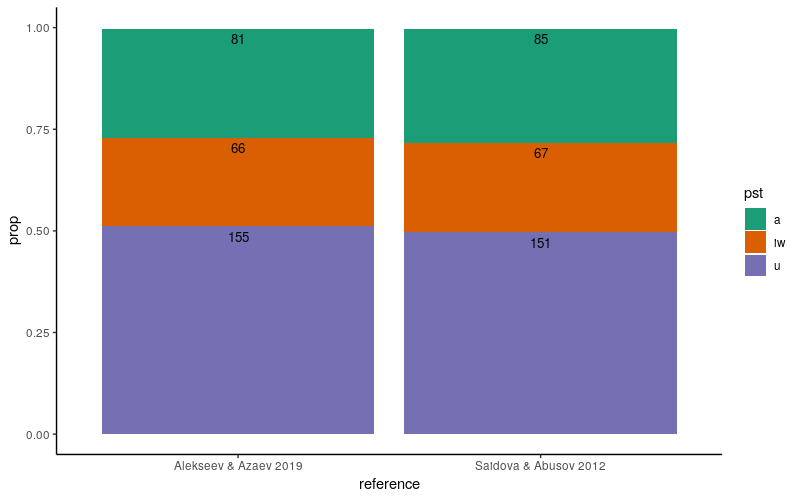
\includegraphics[scale=0.5]{images/pst.png}
\end{figure}
\end{frame}

\begin{frame}{Derived verbs}
Analytic formation of both the habitualis and the aorist with auxiliaries
\begin{itemize}
    \item be: \textit{b-uk'-e}, \textit{b-uk'-a}
    \item become: \textit{b-ah-e}, \textit{b-ah-u}
\end{itemize}
\begin{table}[]
\caption{Derived verbs: inflection}
\centering
\begin{tabular}{l|l|l|l}
      & Infinitive         & Habitualis             & Aorist                 \\ \hline
roar  & \textit{buda-ɬi}   & \textit{buda \textbf{b-uk'-e}}  & \textit{buda \textbf{b-uk'-a}}  \\
bleat & \textit{baʕada-ɬi} & \textit{baʕada \textbf{b-ah-e}} & \textit{baʕada \textbf{b-ah-u}}
\end{tabular}
\end{table}
\end{frame}

\begin{frame}{Causative verbs}
\begin{itemize}
    \item -\textit{o} < \textit{*-a-u} [\textsc{-caus-aor}]
    \item -\textit{mal-e} a reduced form of -\textit{malih-e}?
    \item -\textit{mal-o} rarely found in the data
\end{itemize}
\begin{table}[]
\caption{Causative verbs: inflection}
\centering
\begin{tabular}{l|l|l|l}
         & Infinitive        & Habitualis                & Aorist                    \\ \hline
resettle & \textit{guč-a-j}  & \textit{guč-\textbf{e}}            & \textit{guč-\textbf{o}}            \\
roast    & \textit{žad-a-j}  & \textit{žad-a-j-\textbf{mal-e}}    & \textit{žad-a-j-\textbf{mal-o}}    \\
sew up   & \textit{mik'-a-j} & \textit{mik'-a-j-\textbf{mal-e}}   & \textit{mik'-\textbf{o}}           \\
sew up   & \textit{mik'-a-j} & \textit{mik'-a-j-\textbf{malih-e}} & \textit{mik'-a-j-\textbf{malih-u}}
\end{tabular}
\end{table}
\end{frame}

\begin{frame}{Habitualis in the dictionaries}
\begin{figure}[h]
\centering
\caption{Habitualis}
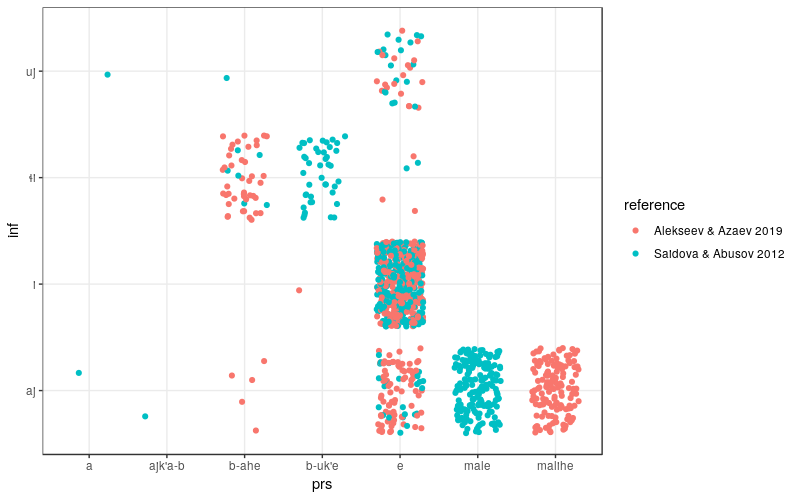
\includegraphics[scale=0.45]{images/infxprs.png}
\end{figure}
\end{frame}

\begin{frame}{Aorist in the dictionaries}
\begin{figure}[h]
\centering
\caption{Aorist}
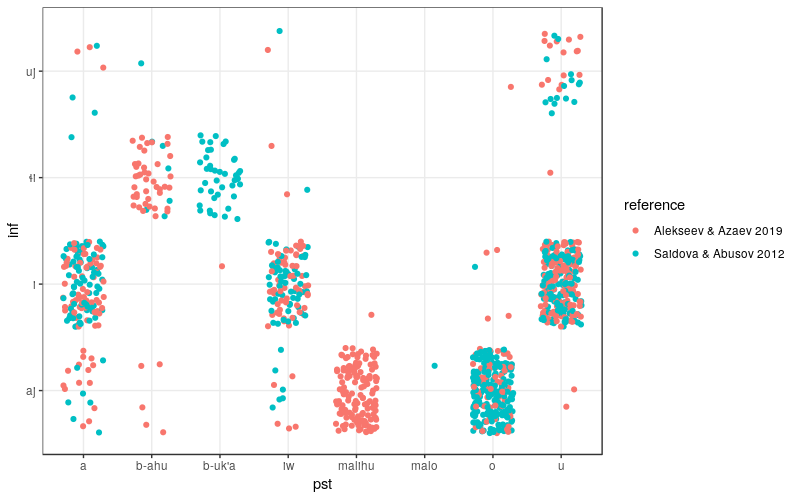
\includegraphics[scale=0.45]{images/infxpst.png}
\end{figure}
\end{frame}

\begin{frame}{Variation}
\begin{itemize}
    \item Basic verbs display little variation in the aorist (and no variation at all in the habitualis)
    \item Most variation is observed for derived and causative verbs:
    \begin{itemize}
        \item Derived verbs: preference for auxiliary `be' in \citet{saidovaabusov2012} vs. `become' in \citet{alekseev2019} \\ BUT it seems that this is just a matter of personal taste for citation forms: examples in the dictionary entries show that both variants are possible
        \item Causative verbs: full (older?) forms -\textit{malih-e} and -\textit{malih-u} in \citet{alekseev2019} vs. reduced form -\textit{mal-e} and synthetic -\textit{o} in \citet{saidovaabusov2012} \\ This might be interpreted as diachronic variation, since the data in \citet{alekseev2019} are older
    \end{itemize}
\end{itemize}
\end{frame}

\section{Discussion}
\begin{frame}{Variation}
The comparison of two dictionaries allowed to identify different types of variation in Botlikh
\begin{itemize}
    \item Phonological variation
    \begin{itemize}
        \item stress patterns
        \item syllable structure
    \end{itemize}
    \item Morphological variation
    \begin{itemize}
        \item nouns: plural suffixes and oblique stem formation
        \item verbs: present (habitualis) and past (aorist) forms
    \end{itemize}
\end{itemize}
Variation seems to affect (to a greater extent) specific groups of words
\begin{itemize}
    \item nouns: borrowings and masdars (both at the phonological and at the morphological level)
    \item verbs: derived and causative
\end{itemize}
\end{frame}

\begin{frame}{Variation}
How do we explain the variation observed?
\begin{itemize}
    \item Idiolectal variation?
    \item Diachronic variation?
    \item Personal preferences of the author?
    \item ...?
\end{itemize}
\end{frame}

\section{Methodological remarks}
\begin{frame}{Methodological remarks}
\begin{itemize}
    \item Two similar datasets collected independently in a small language community approximately in the same time period can nevertheless display considerable variation
    \item This demonstrates the importance of transparency in data collection \\ i.e. metadata on the speakers consulted
    \item And methodological decisions \\ e.g. what is included or not as a separate dictionary entry
\end{itemize}
\end{frame}

\begin{frame}{Methodological remarks}
\begin{itemize}
    \item The availability of comparable material on which quantitative investigations can be conducted is a rare luck for such small languages like Botlikh
    \item This precious information can be used to provide numerical approximations for impressionistic observations reported in the available literature on the language
\end{itemize}
\end{frame}

\begin{frame}{Methodological remarks}
% something about data-driven phonological analysis?
\begin{itemize}
    \item 
\end{itemize}
\end{frame}

\section{Further research}
\begin{frame}{Further research}
\begin{itemize}
    \item Other Avar-Andic dictionaries are being added (Avar, Godoberi, Karata, Tindi, Chamalal, Bagvalal, Akhvakh)
    \item The same procedure of data processing and extraction of grammatical information is being carried out
    \item This will give us the opportunity to conduct comparative analysis at different linguistic levels (phonology, morphology, lexicon) of the different languages of the Avar-Andic branch of EC languages
\end{itemize}
\end{frame}

\section{The end}
\begin{frame}{The end}
\begin{figure}[h]
\centering
\fbox{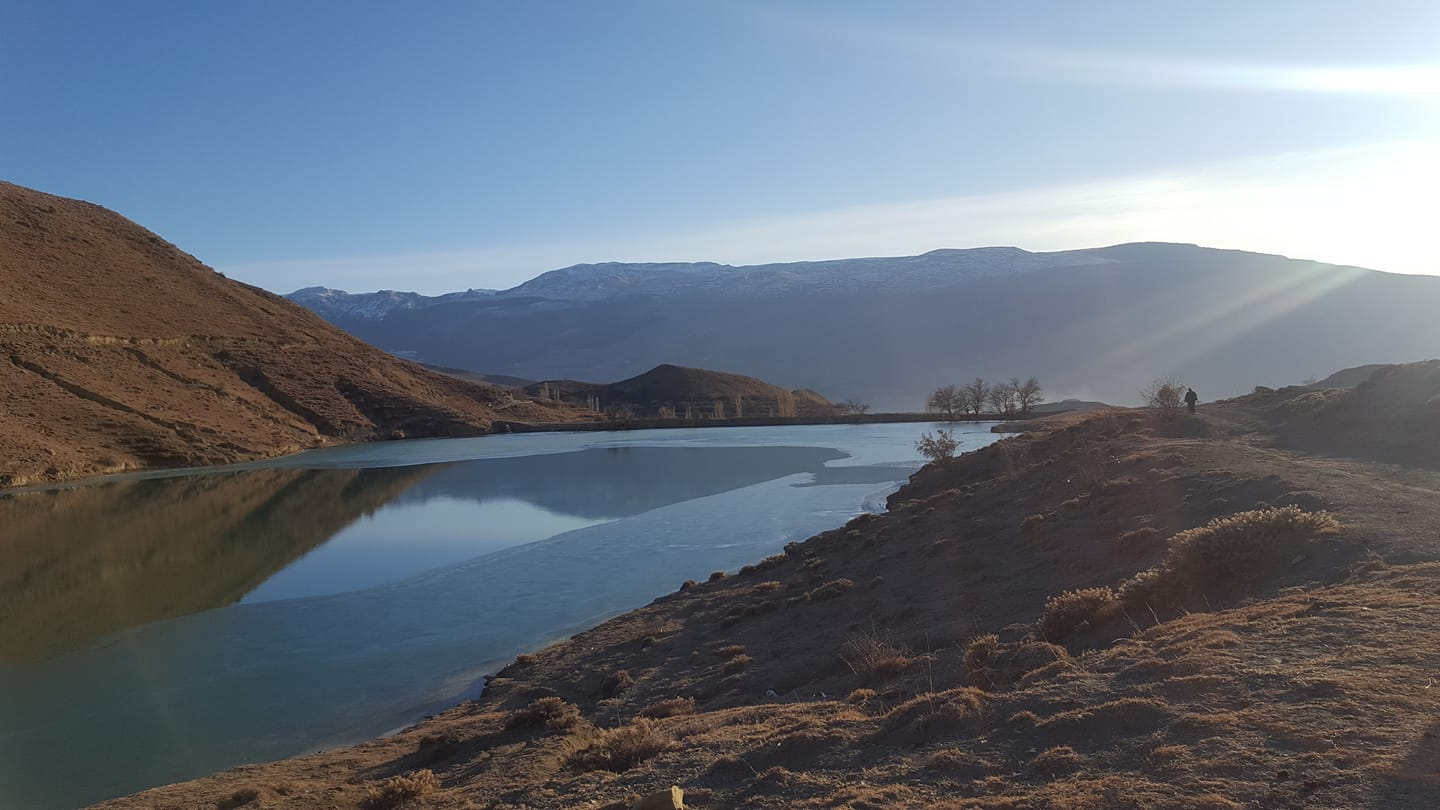
\includegraphics[height=6cm]{images/arqule.jpg}}
\end{figure}
\end{frame}

\section{References}
\begin{frame}[allowframebreaks]{References}
\printbibliography
\end{frame}

\end{document}